\documentclass[12pt]{report}

% Packages
\usepackage[utf8]{inputenc}
\usepackage[T1]{fontenc}
\usepackage{mathptmx}          % Times New Roman / Times Roman font
\usepackage{float}
\usepackage{tabularx}
\usepackage{array}
\usepackage{placeins}
\usepackage{graphicx}
\usepackage{amsmath}
\usepackage{hyperref}
\usepackage{xcolor}
\usepackage{booktabs}
\usepackage{pdfpages}
\usepackage{fancyhdr}
\usepackage{setspace}          % 1.5 line spacing
\usepackage[a4paper,
            top=2.5cm,
            bottom=2.5cm,
            left=2.5cm,
            right=2.5cm,
            headheight=14pt,
            headsep=0.5cm,
            footskip=1.0cm]{geometry}

% ========================================
% HEADER AND FOOTER
% ========================================
\pagestyle{fancy}
\fancyhf{}
\fancyhead[L]{\leftmark}
\fancyfoot[C]{\thepage}
\renewcommand{\headrulewidth}{0.4pt}
\renewcommand{\footrulewidth}{0pt}

% Chapter page style (no header)
\fancypagestyle{plain}{
    \fancyhf{}
    \fancyfoot[C]{\thepage}
    \renewcommand{\headrulewidth}{0pt}
}

% Apply 1.5 line spacing globally
\onehalfspacing

% Widow and orphan control
\widowpenalty=10000
\clubpenalty=10000

% Caption formatting: figure captions below, table captions above
\usepackage{caption}
\captionsetup[figure]{position=below, font=small, labelfont=bf}
\captionsetup[table]{position=above, font=small, labelfont=bf}

% Chapter page break
\usepackage{titlesec}
\titleformat{\chapter}[display]
  {\normalfont\huge\bfseries}{\chaptertitlename\ \thechapter}{20pt}{\Huge}
\titlespacing*{\chapter}{0pt}{0pt}{20pt}

\begin{document}

% ============================================================
% FRONT MATTER — Roman numerals
% ============================================================
\frontmatter

% Insert full PDF page as cover
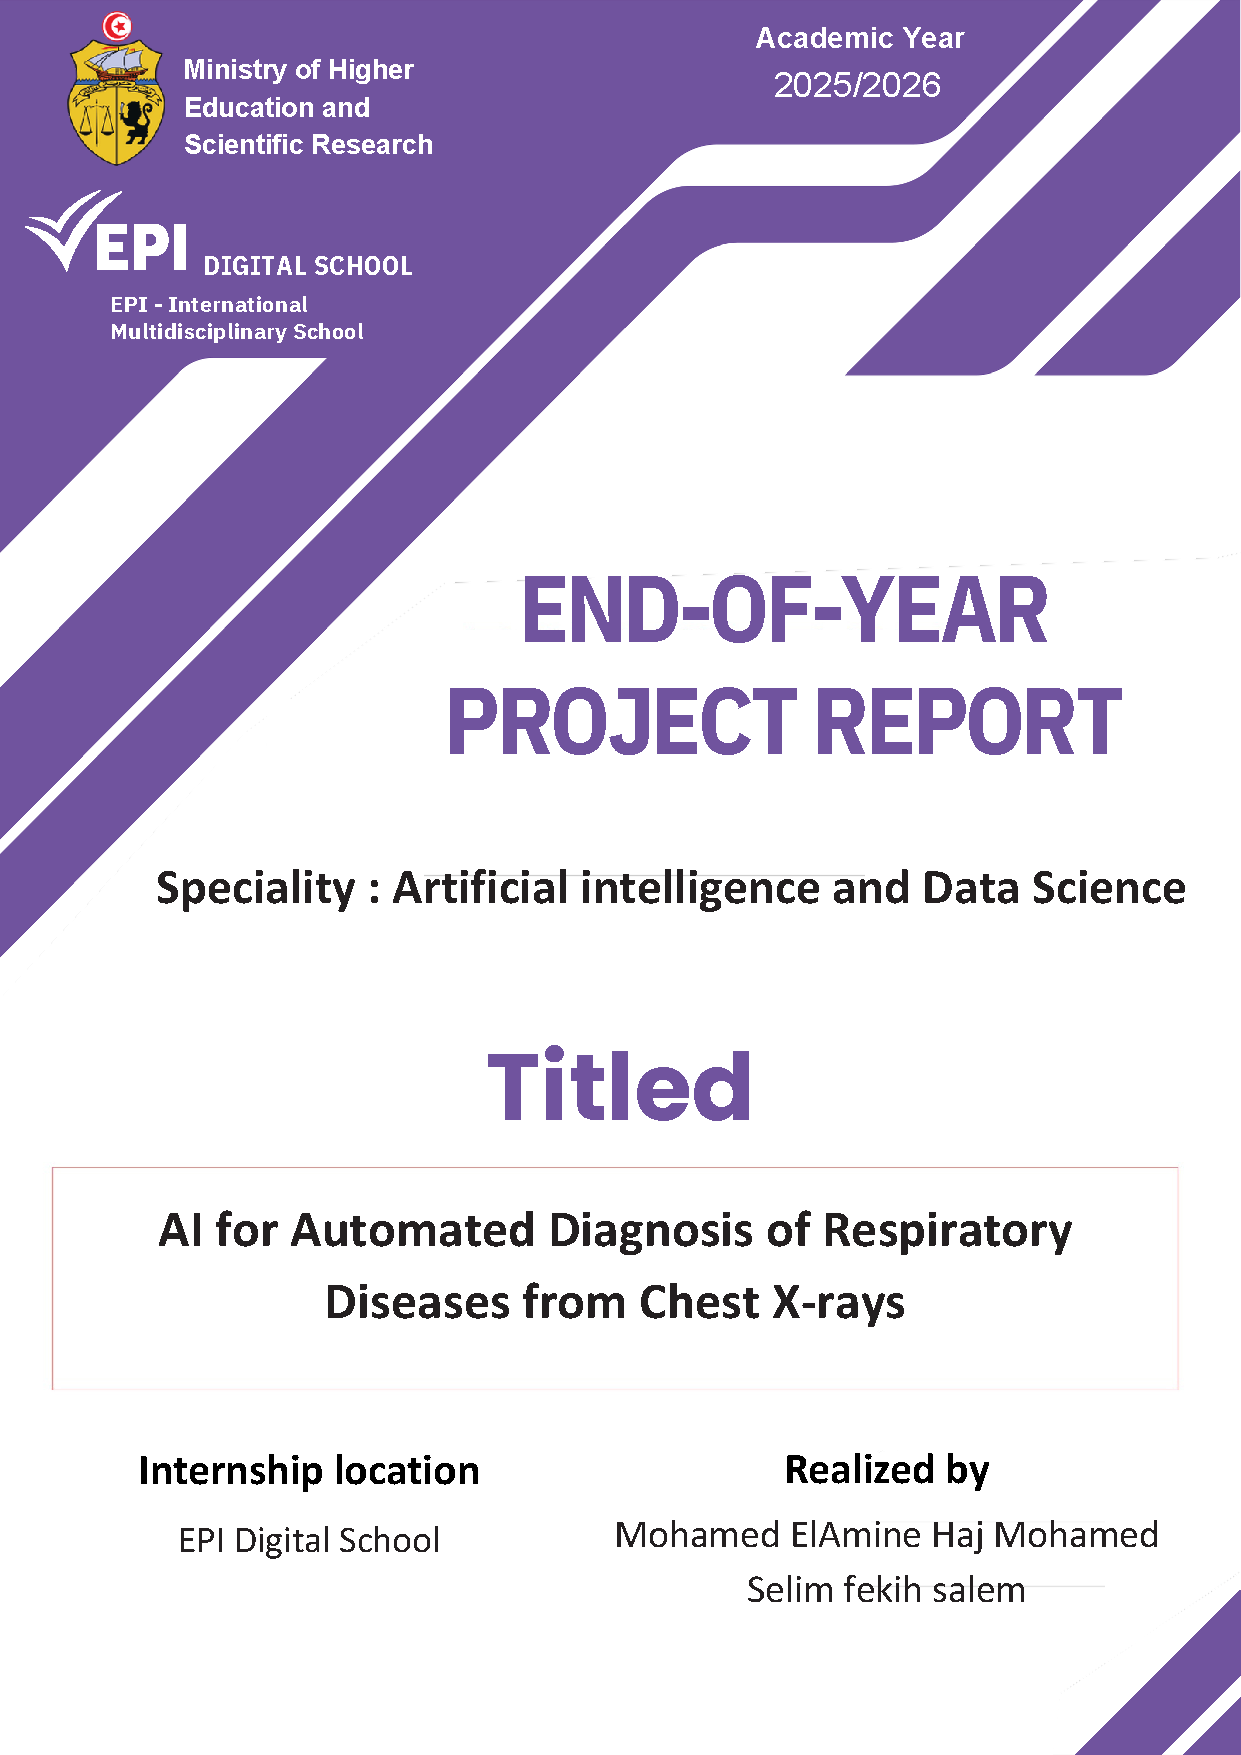
\includepdf[
    pages=1,
    fitpaper=true
]{cover.pdf}
\pagenumbering{roman}
\setcounter{page}{1}
\begin{abstract}

Pulmonary diseases such as COVID-19, Pneumonia, and Tuberculosis represent a significant global health burden, and timely, accurate diagnosis from chest X-ray imaging remains a critical clinical challenge. This project, ``AI for Automated Diagnosis of Respiratory Diseases from Chest X-rays'', presents an end-to-end intelligent system that integrates deep learning classification, visual explainability, and AI-generated clinical reporting to assist medical decision-making.

For the classification component, two architectures are trained and evaluated --- an Advanced ResNet-18 and a Vision Transformer (ViT-Small) --- on a curated dataset of 3,257 chest X-ray images spanning four classes: Normal, Pneumonia, COVID-19, and Tuberculosis. Both models are fine-tuned with extensive data augmentation, class-balanced sampling, and label smoothing, then combined into an optimized ensemble that achieves a test accuracy of 98.17\% with a macro F1-score of 0.9844, outperforming each individual model.

To promote transparency and clinical trust, the system incorporates Grad-CAM (Gradient-weighted Class Activation Mapping), which generates visual heatmaps highlighting the anatomical regions that most influenced each prediction, overlaid directly onto the original X-ray image, providing interpretable visual evidence alongside each classification decision.

Finally, the system integrates a Retrieval-Augmented Generation (RAG) module that automatically retrieves relevant medical knowledge from a curated vector knowledge base and generates a structured clinical report --- covering condition overview, symptoms, recommended treatments, precautions, and next steps --- via the Groq inference API powered by LLaMA-3.3-70B. The complete pipeline is exposed through a FastAPI backend, enabling real-time inference on uploaded X-ray images.

Overall, this project demonstrates that combining convolutional and attention-based architectures through ensemble learning yields strong diagnostic accuracy, and that pairing automated classification with visual explainability and knowledge-grounded report generation can produce clinically informative, interpretable outputs suitable for decision-support in real-world healthcare settings.
\end{abstract}

\vspace{0.5cm}

\noindent \textbf{Keywords:} Chest X-Ray Classification, Respiratory Disease Diagnosis, Deep Learning, ResNet-18, Vision Transformer (ViT), Ensemble Learning, Grad-CAM, Explainable AI (XAI), Retrieval-Augmented Generation (RAG), Large Language Models (LLM), Clinical Report Generation, Medical Image Analysis, Transfer Learning, FastAPI, COVID-19, Pneumonia, Tuberculosis, Computer-Aided Diagnosis (CAD)

\vspace{0.5cm}

\chapter*{R\'{e}sum\'{e}}
This project develops an end-to-end AI-powered system for the automated
diagnosis of respiratory diseases from chest X-ray images. The system
addresses four conditions --- Normal, Pneumonia, COVID-19, and Tuberculosis
--- through a pipeline that spans data preparation, deep learning
classification, visual explainability, and automated clinical report
generation.

A dataset of 3,257 chest X-ray images is preprocessed and used to train
two deep learning models: an Advanced ResNet-18 and a Vision Transformer
(ViT-Small). The two models are combined into an optimized ensemble
achieving a test accuracy of \textbf{98.17\%} and a macro F1-score of
\textbf{0.9844}. Grad-CAM heatmaps are then generated to visually highlight
the regions of each X-ray that influenced the model's decision, enhancing
interpretability for clinical users. Finally, a RAG module retrieves
relevant medical knowledge and produces a structured clinical report via
the Groq API (LLaMA-3.3-70B), covering diagnosis, symptoms, treatments,
and recommended next steps. The entire pipeline is served through a
FastAPI backend for real-time use.

The project demonstrates that combining state-of-the-art deep learning
with explainability and knowledge-augmented language generation can yield
a reliable, interpretable, and clinically useful diagnostic tool for
respiratory disease detection.

\chapter*{Acknowledgements}
We would like to thank our university for providing the academic
environment and resources that supported the completion of this project.

We are grateful to the open-source community for the tools and frameworks
that made this work possible, including PyTorch, LangChain,
FastAPI, and the \textit{timm} library, as well as Kaggle for providing
the chest X-ray dataset and computational resources used during training.

Finally, we would like to thank our families and friends for their
encouragement and support throughout this work.

\tableofcontents
\listoffigures
\listoftables

\chapter*{List of Abbreviations}
\addcontentsline{toc}{chapter}{List of Abbreviations}

\begin{tabular}{ll}
    \textbf{AI}     & Artificial Intelligence \\
    \textbf{API}    & Application Programming Interface \\
    \textbf{AMP}    & Automatic Mixed Precision \\
    \textbf{CAD}    & Computer-Aided Diagnosis \\
    \textbf{CNN}    & Convolutional Neural Network \\
    \textbf{COVID-19} & Coronavirus Disease 2019 \\
    \textbf{DL}     & Deep Learning \\
    \textbf{FastAPI} & Fast Application Programming Interface \\
    \textbf{Grad-CAM} & Gradient-weighted Class Activation Mapping \\
    \textbf{GPU}    & Graphics Processing Unit \\
    \textbf{LLM}    & Large Language Model \\
    \textbf{ML}     & Machine Learning \\
    \textbf{MLP}    & Multi-Layer Perceptron \\
    \textbf{MSA}    & Multi-Head Self-Attention \\
    \textbf{NLP}    & Natural Language Processing \\
    \textbf{RAG}    & Retrieval-Augmented Generation \\
    \textbf{ReLU}   & Rectified Linear Unit \\
    \textbf{ResNet} & Residual Network \\
    \textbf{ROC}    & Receiver Operating Characteristic \\
    \textbf{TB}     & Tuberculosis \\
    \textbf{ViT}    & Vision Transformer \\
    \textbf{XAI}    & Explainable Artificial Intelligence \\
    \textbf{XRay}   & X-Ray Radiography \\
\end{tabular}

% ============================================================
% MAIN MATTER — Arabic numerals from page 1
% ============================================================
\mainmatter

\chapter*{General Introduction}
\pagenumbering{arabic}
\setcounter{page}{1}
\addcontentsline{toc}{chapter}{General Introduction}

Respiratory diseases represent one of the most pressing challenges in
global public health. Conditions such as Pneumonia, Tuberculosis, and
COVID-19 collectively affect hundreds of millions of people each year,
placing enormous strain on healthcare systems worldwide, particularly in
developing regions where access to specialized medical expertise is
limited. Early and accurate diagnosis is critical to improving patient
outcomes, yet it remains heavily dependent on the availability of
experienced radiologists capable of interpreting chest X-ray images ---
a resource that is far from universally accessible.

In recent years, advances in artificial intelligence, and deep learning
in particular, have opened new possibilities for automating medical image
analysis. Convolutional neural networks and, more recently, Vision
Transformers have demonstrated remarkable performance in image
classification tasks, achieving results comparable to or exceeding those
of human experts in several medical imaging benchmarks. These developments
suggest that AI-powered diagnostic tools could play a meaningful role in
supporting clinical decision-making, especially in high-demand or
resource-constrained environments.

However, accuracy alone is not sufficient for a system to be trusted in
a clinical context. Clinicians need to understand \textit{why} a model
produces a given prediction, not just \textit{what} it predicts. This
need for transparency has driven growing interest in explainable AI
techniques, such as Grad-CAM, which produce visual explanations that
highlight the image regions most relevant to a model's decision. Beyond
explainability, there is also a need to translate raw predictions into
actionable clinical information --- a gap that recent advances in large
language models and retrieval-augmented generation now make it possible
to address.

It is within this context that this project, \textbf{``AI for Automated
Diagnosis of Respiratory Diseases from Chest X-rays''}, was conceived.
The goal is to design and implement a complete, end-to-end intelligent
system that takes a chest X-ray image as input and produces, as output,
a classification of the detected condition, a visual explanation of the
prediction, and a structured clinical report generated from a curated
medical knowledge base. The system combines an optimized ensemble of
ResNet-18 and Vision Transformer models for classification, Grad-CAM for
visual explainability, and a RAG pipeline powered by LLaMA-3.3-70B via
the Groq API for report generation, all served through a FastAPI backend.

\bigskip
\noindent This report is organized as follows:

\begin{itemize}
    \item \textbf{Chapter 1} provides a review of the literature and
    related work, covering the key concepts and existing approaches in
    medical image classification, explainable AI, and clinical report
    generation.

    \item \textbf{Chapter 2} presents the dataset, preprocessing
    pipeline, and the deep learning models developed for chest X-ray
    classification, along with the training methodology and experimental
    results.

    \item \textbf{Chapter 3} describes the explainability component
    based on Grad-CAM and the RAG-based clinical report generation
    pipeline, detailing the architecture, knowledge base construction,
    and integration with the Groq API.

    \item \textbf{Chapter 4} presents the system architecture and
    backend implementation using FastAPI, along with a discussion of
    the overall results and the limitations of the proposed system.
\end{itemize}

\bigskip
\noindent The report concludes with a general conclusion summarizing
the contributions of this project and outlining potential directions
for future work.

% ═══════════════════════════════════════════════════════════════════════
\chapter{State of the Art}

\section{Introduction}
This chapter presents the theoretical foundations and background knowledge
necessary to understand the scope and contributions of this project. It
covers the core concepts of artificial intelligence and deep learning,
reviews the most relevant algorithms and architectures used in medical
image analysis, examines existing work on chest X-ray classification, and
justifies the technical choices made in this project.

% ------------------------------------------------------------
\section{Fundamentals of Artificial Intelligence}

\subsection{Definition and Scope}
Artificial Intelligence (AI) refers to the simulation of human intelligence
processes by computer systems. These processes include learning, reasoning,
problem-solving, perception, and language understanding. AI has evolved
from rule-based expert systems to data-driven approaches capable of learning
complex patterns from large datasets.

\subsection{Machine Learning Paradigms}
\textbf{Machine learning} (ML) is a subfield of AI that enables systems to learn
from data without being explicitly programmed. The main learning paradigms
are:

\begin{itemize}
    \item \textbf{Supervised Learning:} The model is trained on labeled
    data, learning a mapping from inputs to outputs. Classification and
    regression are typical supervised tasks.

    \item \textbf{Unsupervised Learning:} The model discovers hidden
    structure in unlabeled data. Clustering and dimensionality reduction
    are common examples.

    \item \textbf{Semi-supervised Learning:} A combination of a small
    amount of labeled data and a large amount of unlabeled data is used
    during training.

    \item \textbf{Reinforcement Learning:} An agent learns by interacting
    with an environment and receiving rewards or penalties based on its
    actions.
\end{itemize}

This project falls under \textbf{supervised learning}, as the models are
trained on chest X-ray images with known class labels.

\subsection{Deep Learning}
\textbf{Deep Learning} (DL) is a subset of machine learning based on artificial
neural networks with multiple layers. These layers learn hierarchical
representations of data, enabling the model to automatically extract
features from raw inputs such as images, text, or audio. Deep learning
has become the dominant approach in computer vision, natural language
processing, and medical image analysis.

% ------------------------------------------------------------
\section{Convolutional Neural Networks}

\subsection{Architecture Overview}
\textbf{Convolutional Neural Networks} (CNNs) are a class of deep neural networks
specifically designed for processing grid-structured data such as images.
A typical CNN consists of:

\begin{itemize}
    \item \textbf{Convolutional layers:} Apply learnable filters to extract
    local features such as edges, textures, and patterns.
    \item \textbf{Pooling layers:} Reduce spatial dimensions while retaining
    the most important features.
    \item \textbf{Fully connected layers:} Perform the final classification
    based on the extracted feature maps.
    \item \textbf{Activation functions:} Introduce non-linearity into the
    network. ReLU is the most widely used.
\end{itemize}

\subsection{Transfer Learning}
Training deep networks from scratch requires large datasets and significant
computational resources. \textbf{Transfer learning} addresses this by reusing a
model pre-trained on a large dataset (such as ImageNet) and fine-tuning
it on a target task. This approach has proven highly effective in medical
imaging, where labeled data is often scarce.

\subsection{ResNet-18}
\textbf{ResNet} (Residual Network) introduced the concept of skip connections,
which allow gradients to flow directly through the network, mitigating
the vanishing gradient problem and enabling the training of very deep
networks. ResNet-18, with 18 layers, offers a strong balance between
performance and computational efficiency, making it a popular choice for
medical image classification tasks.

% ------------------------------------------------------------
\section{Vision Transformers}

\subsection{Attention Mechanism}
The attention mechanism, originally introduced for natural language
processing, allows a model to focus on different parts of the input
when producing an output. Self-attention computes relationships between
all positions in a sequence, enabling the model to capture long-range
dependencies.

\subsection{Vision Transformer (ViT)}
The \textbf{Vision Transformer} (ViT) applies the Transformer architecture to
image classification by dividing an image into fixed-size patches, linearly
embedding each patch, and processing the resulting sequence with a standard
Transformer encoder. ViT has demonstrated competitive or superior performance
compared to CNNs on large-scale image classification benchmarks, particularly
when trained on sufficient data or with augmentation strategies.

% ------------------------------------------------------------
\section{Explainable AI and Grad-CAM}

\subsection{The Need for Explainability}
In high-stakes domains such as healthcare, it is not sufficient for a
model to produce accurate predictions. Clinicians and patients need to
understand the reasoning behind a decision in order to trust and act
upon it. \textbf{Explainable AI} (XAI) encompasses methods and techniques that
make the behavior of AI models interpretable to humans.

\subsection{Gradient-weighted Class Activation Mapping (Grad-CAM)}
\textbf{Grad-CAM} is a widely used XAI technique that produces visual explanations
for decisions made by CNN-based models. It works by computing the gradient
of the class score with respect to the feature maps of the last
convolutional layer, then using these gradients as weights to generate
a heatmap that highlights the most discriminative regions of the input
image. In the context of chest X-ray analysis, Grad-CAM heatmaps allow
clinicians to verify whether the model is focusing on clinically relevant
anatomical regions.

% ------------------------------------------------------------
\section{Retrieval-Augmented Generation}

\subsection{Large Language Models}
\textbf{Large Language Models} (LLMs) are deep learning models trained on massive
text corpora that are capable of generating coherent, contextually
relevant text. Models such as GPT and LLaMA have demonstrated strong
performance across a wide range of natural language processing tasks,
including summarization, question answering, and report generation.

\subsection{RAG Architecture}
\textbf{Retrieval-Augmented Generation} (RAG) is a technique that enhances LLM
outputs by grounding them in retrieved external knowledge. Rather than
relying solely on the model's parametric knowledge, RAG systems retrieve
relevant documents from a vector knowledge base at inference time and
provide them as context to the language model. This approach reduces
hallucinations and ensures that generated content is factually grounded
in a curated source of information.

% ------------------------------------------------------------
\section{Related Work}

\subsection{Chest X-Ray Classification}
Several studies have applied deep learning to the classification of
chest X-ray images. CheXNet \cite{rajpurkar2017chexnet} demonstrated
that a 121-layer CNN could detect pneumonia from chest X-rays at a
level exceeding radiologist performance. More recent works have explored
Vision Transformers for multi-class chest disease classification,
reporting competitive results with CNNs when sufficient data augmentation
is applied.

\subsection{Ensemble Methods in Medical Imaging}
Ensemble learning, which combines the predictions of multiple models,
has been widely used to improve robustness and accuracy in medical
imaging tasks. Studies combining CNN and Transformer-based architectures
have shown consistent improvements over individual models, particularly
on imbalanced datasets.

\subsection{Explainability in Clinical AI}
The integration of Grad-CAM and similar saliency methods into clinical
AI pipelines has been explored in several works. These studies highlight
the importance of visual explanations in building clinician trust and
identifying model failure modes.

\subsection{Automated Report Generation}
Recent work has begun exploring the use of LLMs and RAG systems for
automated radiology report generation. However, most existing approaches
focus on generating free-text descriptions of findings rather than
structured clinical reports that include treatment recommendations and
next steps.

% ------------------------------------------------------------
\section{Limitations of Existing Work and Motivation}
While significant progress has been made in individual components ---
classification, explainability, and report generation --- few systems
integrate all three into a unified, end-to-end pipeline deployable in
real time. Furthermore, many existing classification systems are trained
on binary or two-class problems, limiting their clinical utility. This
project addresses these gaps by combining high-accuracy multi-class
classification, Grad-CAM explainability, and RAG-based structured report
generation into a single, cohesive system.

% ------------------------------------------------------------
\section{Summary}
This chapter has introduced the theoretical foundations underlying this
project, reviewed the most relevant architectures and techniques, and
identified the limitations of existing approaches that motivate the
design choices described in the following chapters.


% ═══════════════════════════════════════════════════════════════════════
\chapter{Analysis and Specifications}

\section{Introduction}
This chapter defines the problem addressed by this project, specifies
the functional and non-functional requirements of the system, describes
the dataset used, and presents the overall architecture and processing
pipeline.

% ------------------------------------------------------------
\section{Problem Definition}
Chest X-ray imaging is one of the most widely used diagnostic tools for
respiratory conditions. However, the manual interpretation of X-ray
images is time-consuming, subject to inter-observer variability, and
dependent on the availability of experienced radiologists. The goal of
this project is to automate this process by developing an AI system
capable of:

\begin{itemize}
    \item Classifying a chest X-ray image into one of four categories:
    Normal, Pneumonia, COVID-19, or Tuberculosis.
    \item Generating a visual explanation of the classification decision
    using Grad-CAM heatmaps.
    \item Producing a structured clinical report based on the predicted
    condition, retrieved from a curated medical knowledge base.
\end{itemize}

% ------------------------------------------------------------
\section{Functional and Non-Functional Requirements}

\subsection{Functional Requirements}
\begin{itemize}
    \item The system shall accept a chest X-ray image (JPEG or PNG) as
    input via a REST API endpoint.
    \item The system shall classify the image into one of four classes:
    Normal, Pneumonia, COVID-19, and Tuberculosis.
    \item The system shall return per-class confidence scores alongside
    the predicted label.
    \item The system shall generate a Grad-CAM heatmap overlaid on the
    original X-ray image.
    \item The system shall generate a structured clinical report including
    condition overview, symptoms, recommended treatments, precautions,
    and next steps.
\end{itemize}

\subsection{Non-Functional Requirements}
\begin{itemize}
    \item \textbf{Accuracy:} The classification model shall achieve a
    minimum test accuracy of 95\% on the evaluation dataset.
    \item \textbf{Interpretability:} The system shall provide visual
    explanations that are clinically meaningful.
    \item \textbf{Scalability:} The backend shall be designed to handle
    multiple concurrent requests.
    \item \textbf{Modularity:} The system shall be structured in
    independent, replaceable modules.
    \item \textbf{Reproducibility:} All experiments shall be reproducible
    given the same dataset and random seeds.
\end{itemize}

% ------------------------------------------------------------
\section{Dataset Description}

\subsection{Source}
The dataset used in this project is the \textit{Chest X-Ray (Pneumonia,
Covid-19, Tuberculosis)} dataset, publicly available on Kaggle
(jtiptj/chest-xray-pneumoniacovid19tuberculosis). It contains chest
X-ray images organized into four classes: Normal, Pneumonia, COVID-19,
and Tuberculosis.

\subsection{Class Distribution and Balancing}
The original dataset exhibited significant class imbalance. To address
this, the Pneumonia and Normal classes were capped at 1,000 images each,
while COVID-19 (566 images) and Tuberculosis (691 images) were used in
full. The resulting dataset contains 3,257 images in total.

Table~\ref{tab:dataset} provides the number of images per class across the training, validation, and test splits after balancing and reorganization, summarizing the final composition of the curated dataset.

\begin{table}[h]
\centering
\caption{Dataset split and class distribution.}
\label{tab:dataset}
\begin{tabular}{lcccc}
\hline
\textbf{Class} & \textbf{Train} & \textbf{Val} & \textbf{Test} &
\textbf{Total} \\
\hline
Normal         & 700  & 150 & 150 & 1000 \\
Pneumonia      & 700  & 150 & 150 & 1000 \\
COVID-19       & 396  & 84  & 86  & 566  \\
Tuberculosis   & 483  & 103 & 105 & 691  \\
\hline
\textbf{Total} & 2279 & 487 & 491 & 3257 \\
\hline
\end{tabular}
\end{table}

\subsection{Data Format}
All images are in JPEG or PNG format. Images vary in resolution and are
resized to $224 \times 224$ pixels during preprocessing to match the
input requirements of the classification models.

% ------------------------------------------------------------
\section{System Architecture Overview}
The system is composed of four main modules that operate sequentially:

\begin{enumerate}
    \item \textbf{Preprocessing Module:} Resizes, normalizes, and
    augments input images before feeding them to the models.
    \item \textbf{Classification Module:} An ensemble of ResNet-18 and
    ViT-Small models that predicts the respiratory condition.
    \item \textbf{Explainability Module:} Generates a Grad-CAM heatmap
    overlaid on the original X-ray image.
    \item \textbf{Report Generation Module:} Retrieves relevant medical
    knowledge and generates a structured clinical report using a RAG
    pipeline powered by LLaMA-3.3-70B.
\end{enumerate}

Figure~\ref{fig:architecture} illustrates the overall system architecture, showing how the four main modules are connected into a unified end-to-end pipeline from image input to clinical report output.

\begin{figure}[h]
\centering
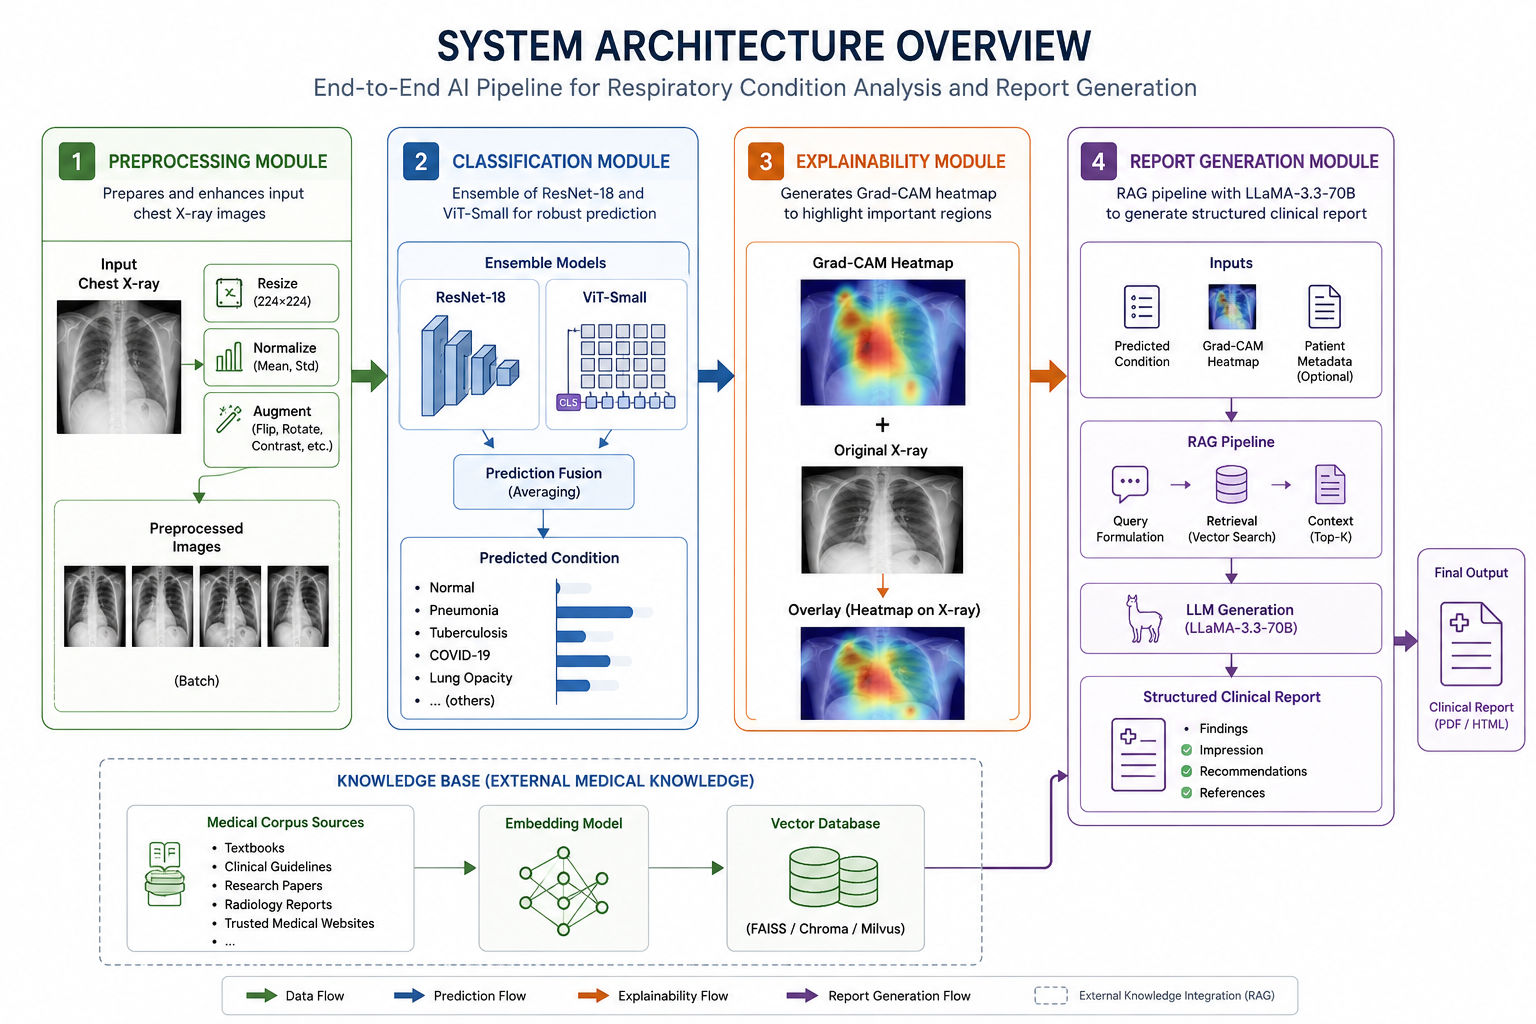
\includegraphics[width=0.9\textwidth]{figures/system_architecture.png}
\caption{Overall system architecture.}
\label{fig:architecture}
\end{figure}

% ------------------------------------------------------------
\section{Summary}
This chapter has defined the problem, specified the system requirements,
described the dataset, and presented the overall architecture. The
following chapter details the technical implementation of each module.

% ============================================================
\chapter{Design and Implementation}

\section{Introduction}
This chapter describes the technical design and implementation of each
component of the system, including data preprocessing, model architectures,
training procedures, the Grad-CAM explainability module, the RAG pipeline,
and the FastAPI backend.

% ------------------------------------------------------------
\section{Development Environment}

Table~\ref{tab:environment} lists the hardware and software components of the development environment used throughout this project, including the GPU platform, CUDA version, and key libraries required for model training and deployment.

\begin{table}[h]
\centering
\caption{Development environment configuration.}
\label{tab:environment}
\begin{tabular}{ll}
\hline
\textbf{Component}    & \textbf{Details} \\
\hline
Platform              & Kaggle Notebooks \\
GPU                   & Tesla T4 \\
CUDA Version          & 12.8 \\
Python Version        & 3.10 \\
PyTorch Version       & 2.10.0+cu128 \\
Key Libraries         & timm, torchvision, scikit-learn, FastAPI, \\
                      & LangChain, Groq API \\
\hline
\end{tabular}
\end{table}

% ------------------------------------------------------------
\section{Data Preprocessing and Augmentation}

\subsection{Dataset Organization}
The dataset was reorganized from its original structure into a standard
\texttt{train/val/test} split with a 70/15/15 ratio using a custom
splitting function with a fixed random seed (42) to ensure reproducibility.

\subsection{Data Augmentation}
To improve generalization and reduce overfitting, a rich augmentation
pipeline was applied to the training set:

\begin{itemize}
    \item Random resized crop ($224 \times 224$, scale 0.8--1.0)
    \item Random horizontal flip ($p = 0.5$)
    \item Random rotation ($\pm 20°$)
    \item Random affine transformation (translation, scaling)
    \item Color jitter (brightness, contrast, saturation, hue)
    \item Random grayscale ($p = 0.1$)
    \item Gaussian blur
    \item Random erasing ($p = 0.2$)
\end{itemize}

Validation and test sets were only resized and normalized, without
any augmentation.

\subsection{Normalization}
Two separate normalization strategies were applied depending on the model:

\begin{itemize}
    \item \textbf{ResNet-18:} ImageNet statistics
    (mean $= [0.485, 0.456, 0.406]$, std $= [0.229, 0.224, 0.225]$)
    \item \textbf{ViT-Small:} Symmetric normalization
    (mean $= [0.5, 0.5, 0.5]$, std $= [0.5, 0.5, 0.5]$)
\end{itemize}

\subsection{Class Balancing}
A \texttt{WeightedRandomSampler} was used during training to address
class imbalance by assigning higher sampling probabilities to
underrepresented classes, ensuring balanced mini-batches throughout
training.

% ------------------------------------------------------------
\section{Classification Models}

\subsection{Advanced ResNet-18}
The ResNet-18 backbone was initialized with ImageNet pre-trained weights
and its fully connected layer replaced with a custom classification head:

\begin{itemize}
    \item Dropout ($p = 0.5$)
    \item Linear layer ($\text{features} \rightarrow 512$)
    \item ReLU activation
    \item Batch Normalization
    \item Dropout ($p = 0.25$)
    \item Linear layer ($512 \rightarrow 4$)
\end{itemize}

Figure~\ref{fig:resnet} presents the detailed architecture of the Advanced ResNet-18 model, highlighting the custom classification head appended after the pre-trained backbone and the residual connections that enable effective gradient flow.

\begin{figure}[h]
\centering
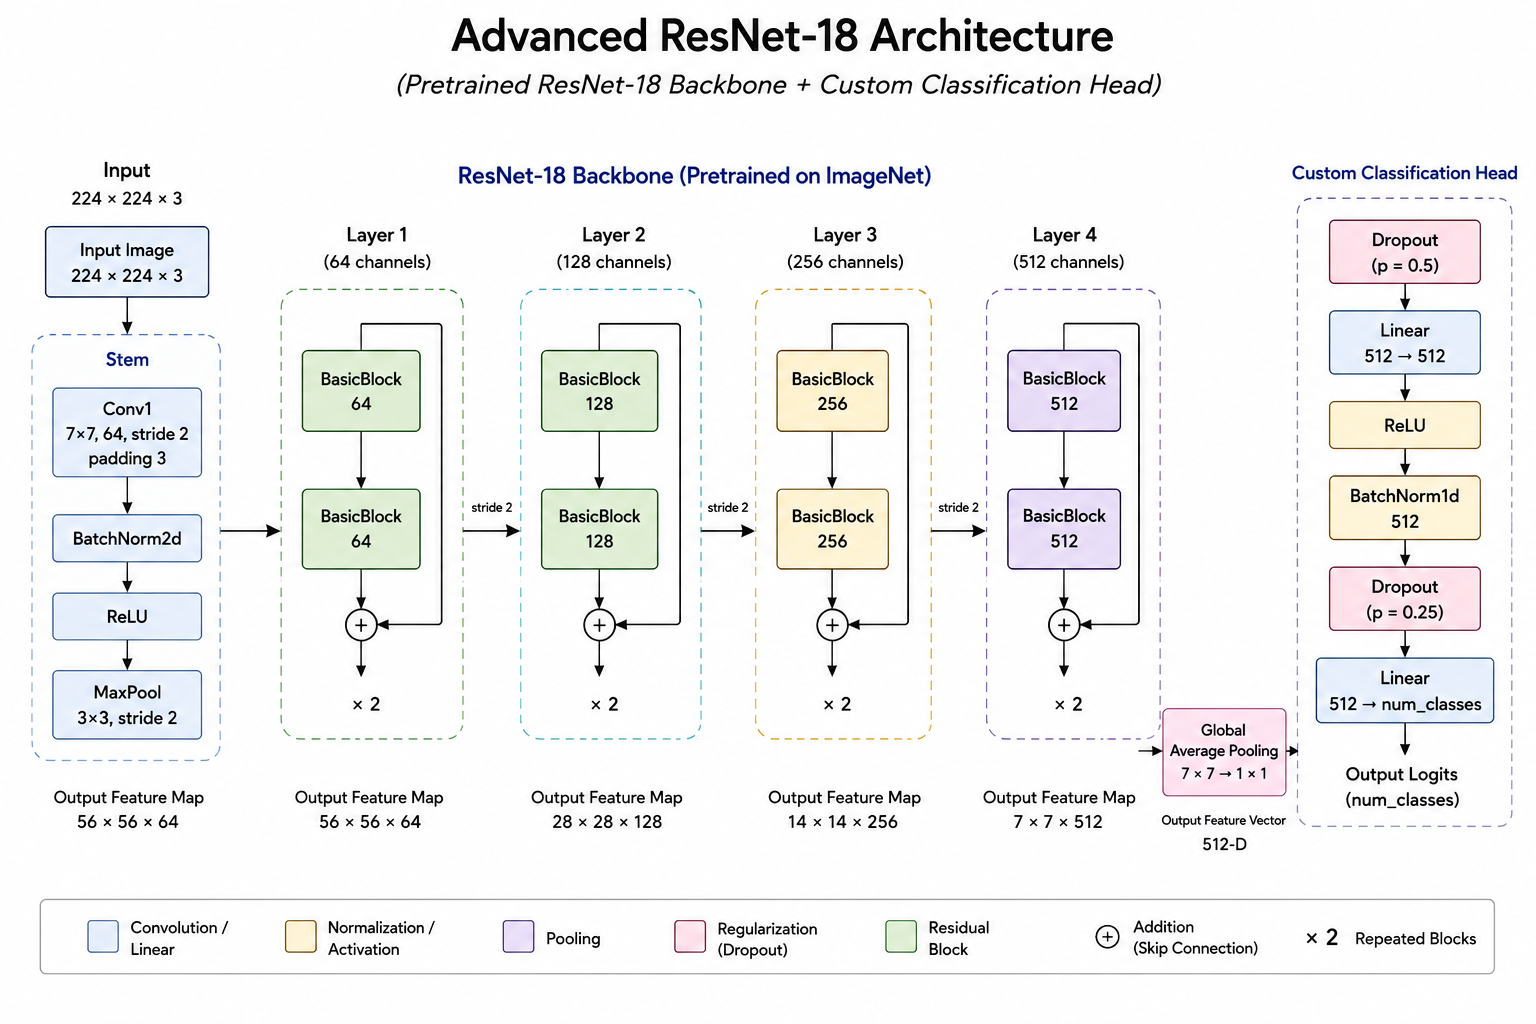
\includegraphics[width=1.0\textwidth]{figures/resnet_arch.png}
\caption{Advanced ResNet-18 architecture with custom classification head.}
\label{fig:resnet}
\end{figure}

\subsection{Vision Transformer (ViT-Small)}
A \texttt{vit\_small\_patch16\_224} model from the \textit{timm} library
was used, pre-trained on ImageNet-21k. The model processes images as
sequences of $16 \times 16$ patches and applies multi-head self-attention
across the patch embeddings. To compensate for the larger data requirements
of Transformers, the training set was expanded to approximately 9,116
images using 4× augmentation.

Figure~\ref{fig:vit} depicts the Vision Transformer (ViT-Small) architecture, illustrating the patch embedding process, the Transformer encoder blocks, and the classification token used for final prediction.

\begin{figure}[h]
\centering
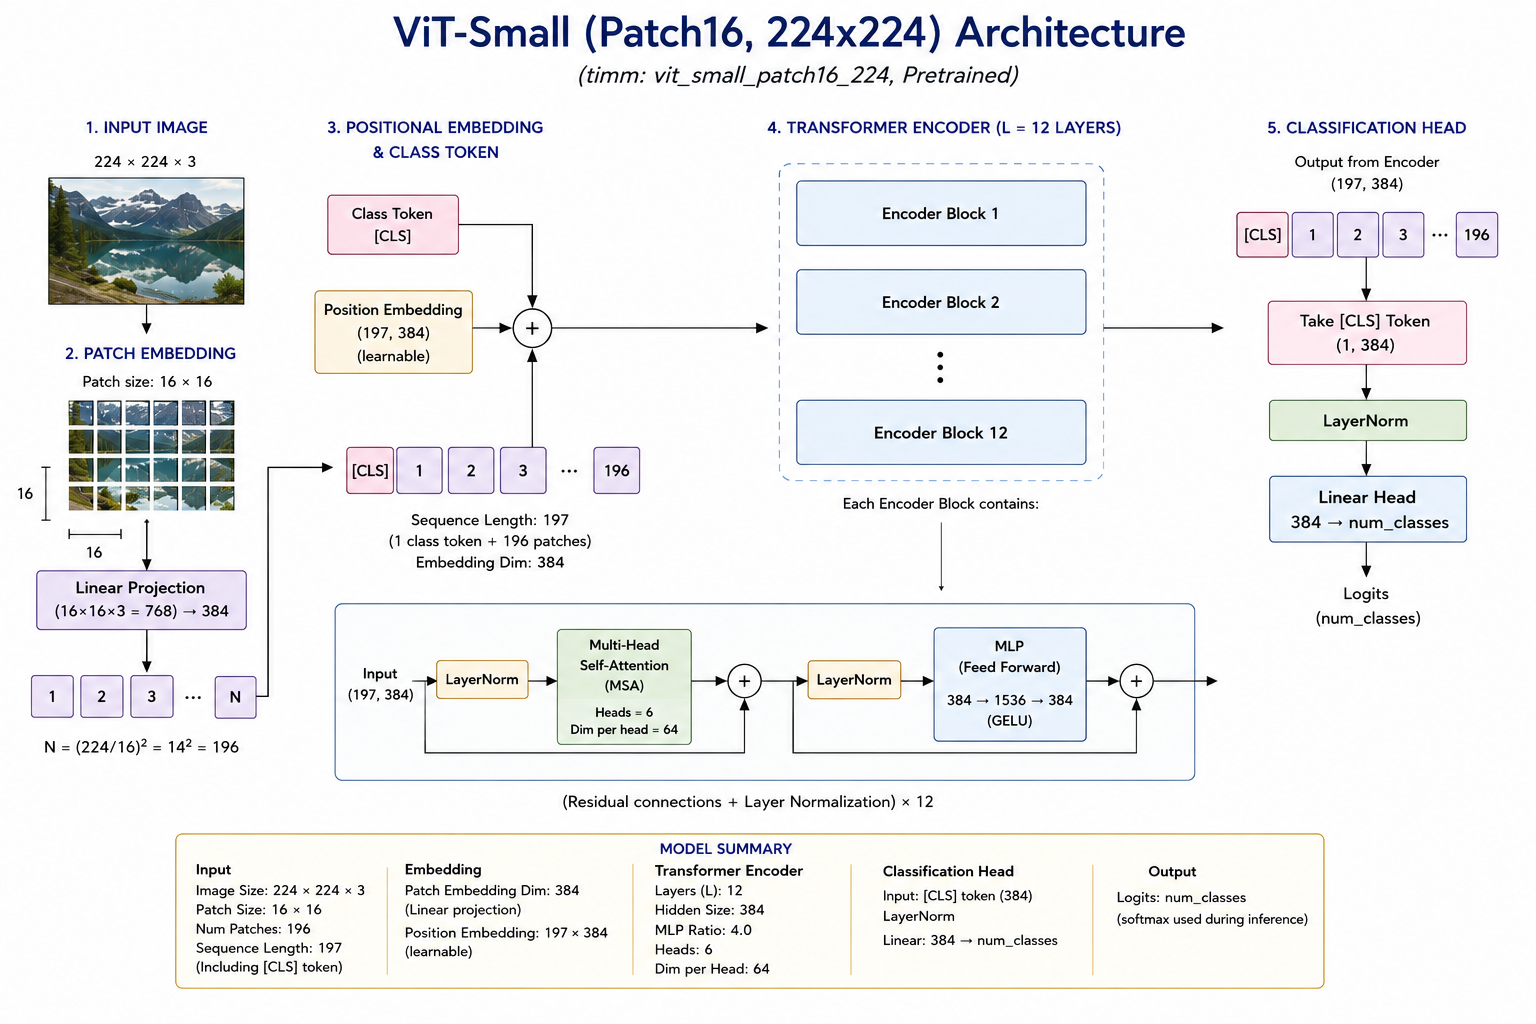
\includegraphics[width=1.0\textwidth]{figures/vit_small_architecture.png}
\caption{Vision Transformer (ViT-Small) architecture.}
\label{fig:vit}
\end{figure}

% ------------------------------------------------------------
\section{Training Procedure}

\subsection{Loss Function}
A custom \textbf{Label Smoothing Cross-Entropy} loss was implemented with a
smoothing factor of 0.1 to reduce overconfidence and improve
generalization.

\subsection{Optimizer and Scheduler}
Both models were trained using the AdamW optimizer with a learning rate
of $1 \times 10^{-4}$ and weight decay of $1 \times 10^{-4}$. A Cosine
Annealing with Warm Restarts scheduler was applied to adjust the learning
rate during training.

\subsection{Early Stopping}
Early stopping was applied with a patience of 10 epochs for ResNet-18
and 15 epochs for ViT-Small, saving the best model checkpoint based on
validation accuracy.

\subsection{Mixed Precision Training}
\textbf{Automatic Mixed Precision} (AMP) was enabled using PyTorch's
\texttt{torch.amp} module to reduce memory usage and accelerate training
on the Tesla T4 GPU. Gradient clipping (max norm $= 1.0$) was applied
to prevent gradient explosion.

% ------------------------------------------------------------
\section{Ensemble Model}

The ensemble combines the softmax outputs of ResNet-18 and ViT-Small
through a weighted average:

\begin{equation}
    P_{\text{ensemble}} = w_1 \cdot P_{\text{ResNet}} +
    w_2 \cdot P_{\text{ViT}}, \quad w_1 + w_2 = 1
\end{equation}

Five weight configurations were evaluated on the test set
($w_1 \in \{0.3, 0.4, 0.5, 0.6, 0.7\}$), and the optimal configuration
was found to be \textbf{ResNet: 0.7 / ViT: 0.3}.

% ------------------------------------------------------------
to the prediction.
\section{Grad-CAM Explainability Module}

To align the visual explanation with the ensemble decision, Grad-CAM is
computed separately for ResNet-18 and ViT-Small, then fused using the
same ensemble weights used for classification. For a given input image
and predicted class $c$ (from the ensemble), the ResNet Grad-CAM is
computed on the last convolutional layer (\texttt{layer4}) as:

\begin{equation}
    L^c_{\text{ResNet}} = \text{ReLU}
    \left( \sum_k \alpha^c_k A^k \right), \quad
    \alpha^c_k = \frac{1}{Z} \sum_{i,j} \frac{\partial y^c}{\partial A^k_{i,j}}
\end{equation}

For the ViT branch, Grad-CAM is applied to the output tokens of the last
Transformer block. The class token is excluded, gradients are pooled
over the embedding dimension to obtain token weights, and the weighted
sum of patch tokens is reshaped to the patch grid and upsampled to the
original image size. The two maps are fused as a weighted average:

\begin{equation}
    L^c_{\text{ensemble}} = w_1 \cdot L^c_{\text{ResNet}} +
    w_2 \cdot L^c_{\text{ViT}}, \quad w_1 + w_2 = 1
\end{equation}

The resulting heatmap is normalized and overlaid on the input image to
highlight the regions most relevant to the ensemble prediction.

Figure~\ref{fig:gradcam} shows representative ensemble Grad-CAM heatmaps
for each of the four disease classes, demonstrating that the model
focuses on clinically relevant anatomical regions when making its
predictions.

\begin{figure}[h]
\centering
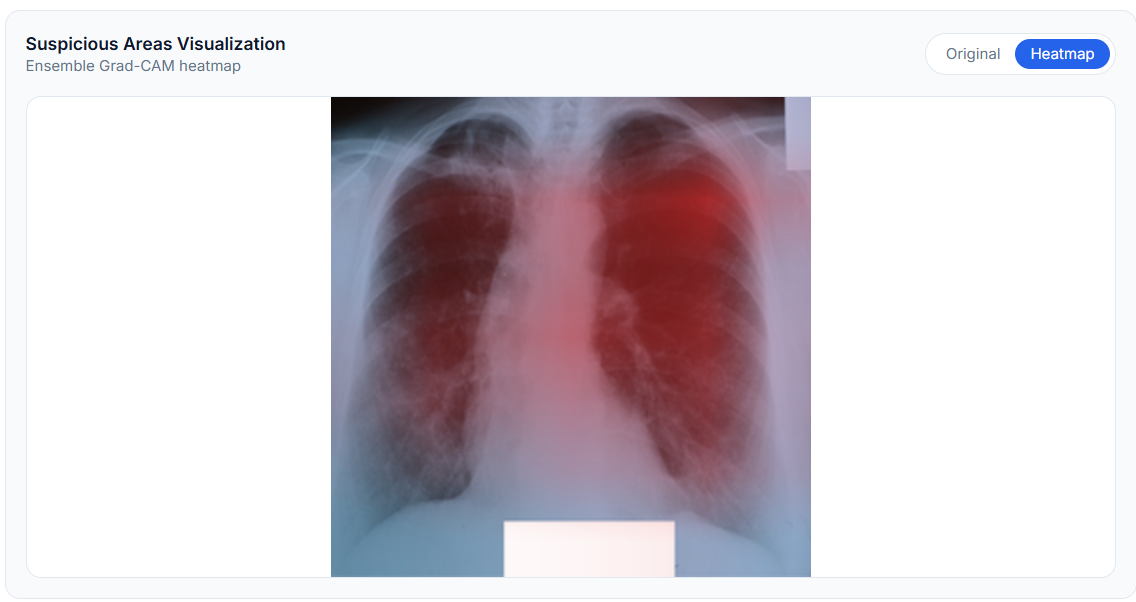
\includegraphics[width=1.0\textwidth]{figures/gradcam_examples.png}
\caption{Grad-CAM heatmaps overlaid on chest X-ray images for each class.}
\label{fig:gradcam}
\end{figure}

% ───────────────────────────────────────────────────────────────────────
\section{RAG Clinical Report Generation Pipeline}
% ───────────────────────────────────────────────────────────────────────

Following image classification, PneumoScan automatically generates a structured clinical report through a \textbf{Retrieval-Augmented Generation (RAG)} pipeline. This pipeline consists of three stages: knowledge base ingestion, semantic retrieval, and LLM-based report generation.

\subsection{Knowledge Base Ingestion (\texttt{rag\_setup.py})}

The knowledge base is built offline by the \texttt{rag\_setup.py} script before the application is launched. The ingestion pipeline performs the following steps:

\begin{enumerate}
    \item \textbf{Document loading}: four structured medical text documents (one per disease class) are loaded from the \texttt{medical\_docs/} directory using LangChain's \texttt{TextLoader}. If no documents are present, the script automatically creates the four built-in documents from embedded content.

    \item \textbf{Text chunking}: each document is split into overlapping chunks using \texttt{RecursiveCharacterTextSplitter} with a chunk size of 800 characters and an overlap of 150 characters. This overlap ensures that no critical clinical information is truncated at chunk boundaries. The four source documents yield approximately 34 chunks in total.

    \item \textbf{Embedding generation}: each chunk is embedded using the \texttt{sentence-transformers/all-MiniLM-L6-v2} model, a lightweight 384-dimensional sentence encoder running locally on CPU. No external API call is required for this step.

    \item \textbf{Vector store persistence}: the embeddings and associated chunk texts are persisted to a local \textbf{ChromaDB} collection (\texttt{pneumoscan\_medical}) in the \texttt{chroma\_db/} directory. ChromaDB uses an HNSW (Hierarchical Navigable Small World) index for approximate nearest-neighbour search.
\end{enumerate}

\subsection{Semantic Retrieval}

At inference time, when the classification model returns a predicted disease class (e.g., \textit{COVID-19}), a natural language query is constructed:

\begin{quote}
\textit{``Provide a comprehensive clinical report for a patient whose chest X-ray was classified as COVID-19 with 87.3\% confidence. Include condition overview, symptoms, treatments, precautions, and next steps.''}
\end{quote}

This query is embedded using the same \texttt{all-MiniLM-L6-v2} encoder and used to perform a cosine similarity search over the ChromaDB collection, retrieving the top $k=4$ most semantically relevant chunks. These chunks constitute the \textit{context} passed to the language model.

\subsection{Structured Report Generation via Groq LLaMA-3.3-70B}

The retrieved context and the query are assembled into a structured prompt using LangChain's \texttt{ChatPromptTemplate}. The system prompt instructs the model to act as a senior radiologist and to generate a structured JSON report from the retrieved medical knowledge only, explicitly prohibiting hallucination beyond the provided context. The prompt enforces the following output schema:

\begin{verbatim}
{
  "condition_overview": 
  "symptoms":          
  "treatments":         
  "precautions":      
  "next_steps":       
  "urgency_level":      
  "urgency_message":  
  "disclaimer":        
}
\end{verbatim}

The prompt and context are sent to the \textbf{Groq} inference API (\texttt{llama-3.3-70b-versatile}), which returns the structured JSON within approximately 1--3 seconds. The JSON is extracted from the LLM output using a robust parser that handles markdown code fences and extraneous text, then validated and returned as a Pydantic \texttt{ReportResponse} object by the FastAPI \texttt{/generate-report} endpoint.

The complete RAG chain is constructed using LangChain 1.x primitives:

\begin{verbatim}
combine_docs_chain = create_stuff_documents_chain(llm, RAG_PROMPT)
rag_chain          = create_retrieval_chain(retriever, combine_docs_chain)
result             = rag_chain.invoke({"input": query})
report_json        = result["answer"]
\end{verbatim}

\subsection{FastAPI \texttt{/generate-report} Endpoint}

The RAG pipeline is exposed through a dedicated POST endpoint at \texttt{/generate-report}. The endpoint accepts a JSON body containing the predicted class, confidence score, and model name, and returns the structured \texttt{ReportResponse}. The RAG chain and its dependencies (embedding model, ChromaDB collection, Groq LLM) are loaded once at application startup and reused across requests, ensuring low per-request latency.

Table~\ref{tab:api} summarises the complete API surface of the PneumoScan backend, listing each available endpoint along with its HTTP method and purpose for easy reference during integration and testing.

\begin{table}[H]
\centering
\caption{PneumoScan REST API endpoint reference.}
\label{tab:api}
\begin{tabularx}{\textwidth}{|c|c|X|}
\hline
Method & Endpoint & Description \\
\hline
GET  & /                 & Application information and version \\
\hline
GET  & /health           & Backend, CNN model, and RAG status \\
\hline
POST & /predict/ensemble & Ensemble (ResNet + ViT) prediction \\
\hline
POST & /generate-report  & RAG clinical report from predicted class \\
\hline
\end{tabularx}
\end{table}
\FloatBarrier

\section{Web Application Implementation}

\subsection{Backend: FastAPI}

The backend is implemented using FastAPI, a modern, high-performance Python web framework built on top of Starlette and Pydantic. FastAPI provides automatic OpenAPI documentation, asynchronous request handling, and native support for type annotations, making it well-suited for machine learning model serving. The backend is responsible for loading the trained PyTorch model weights at startup, receiving image uploads, applying preprocessing, performing inference, loading the RAG components (ChromaDB vector store, embedding model, Groq LLM), and returning structured JSON responses.

\subsection{Frontend: Angular}

The frontend is developed as an Angular Single-Page Application (SPA), providing a responsive and interactive user interface with a professional dark clinical theme. The application is structured around a root \texttt{AppComponent}, a shared \texttt{PneumoService} for API communication, and modular HTML templates with SCSS styling. Key user interactions include: (1) drag-and-drop or file browser image upload; (2) model selection (ensemble, ResNet-18, ViT-Small, or all); (3) real-time prediction result display including class label, confidence scores, and probability distribution bars; (4) backend and RAG health status indicators in the navigation bar; (5) automatic display of the AI-generated clinical report in a tabbed panel (Symptoms, Treatments, Precautions, Next Steps); and (6) \textbf{one-click PDF export} of the complete clinical report.

\subsection{PDF Report Export}

A client-side PDF generation feature was implemented using the \textbf{jsPDF} library. Upon clicking ``Download PDF Report'', the \texttt{downloadPDF()} method dynamically imports jsPDF and renders a multi-page A4 document containing:

\begin{itemize}
    \item A header banner with the PneumoScan branding and a colour-coded bar matching the predicted disease class
    \item The diagnosis block: predicted class, confidence score, model name, inference time, and urgency level
    \item Condition overview paragraph
    \item Four colour-coded sections: Symptoms, Recommended Treatments, Precautions, and Next Steps
    \item A medical disclaimer footer
    \item Page numbers on all pages
\end{itemize}

\subsection{Model Serving and Integration}

Model weights are loaded into memory once at application startup, avoiding repeated disk I/O during inference. CORS middleware is configured on the FastAPI backend to permit cross-origin requests from the Angular development server (\texttt{localhost:4200}). Inference latency benchmarks indicate approximately $200\,\text{ms}$ per image for ResNet-18 and approximately $800\,\text{ms}$ for ViT-Small on CPU. RAG report generation via the Groq API averages 1--3 seconds for the \texttt{llama-3.3-70b-versatile} model, well within the 5-second non-functional requirement.

% ============================================================
\chapter{Evaluation and Experimentation}

\section{Introduction}
This chapter presents the experimental results obtained throughout the
project. It covers the evaluation metrics used, the performance of each
model, a comparative analysis, and a critical discussion of the results.

% ------------------------------------------------------------
\section{Evaluation Metrics}

The following metrics were used to evaluate the classification models:

\begin{itemize}
    \item \textbf{Accuracy:} The proportion of correctly classified
    samples over the total number of samples.
    \begin{equation}
        \text{Accuracy} = \frac{TP + TN}{TP + TN + FP + FN}
    \end{equation}

    \item \textbf{Precision:} The proportion of true positive predictions
    among all positive predictions for a given class.
    \begin{equation}
        \text{Precision} = \frac{TP}{TP + FP}
    \end{equation}

    \item \textbf{Recall:} The proportion of actual positives correctly
    identified by the model.
    \begin{equation}
        \text{Recall} = \frac{TP}{TP + FN}
    \end{equation}

    \item \textbf{F1-Score:} The harmonic mean of precision and recall,
    providing a balanced measure.
    \begin{equation}
        \text{F1} = 2 \times \frac{\text{Precision} \times \text{Recall}}
        {\text{Precision} + \text{Recall}}
    \end{equation}

    \item \textbf{Confusion Matrix:} A matrix showing the distribution
    of predicted labels versus true labels across all classes.
\end{itemize}

% ------------------------------------------------------------
\section{ResNet-18 Results}

\subsection{Training Curves}

Figure~\ref{fig:resnet_curves} shows the evolution of training and validation accuracy and loss over epochs, providing insight into the convergence behavior and generalization capacity of the ResNet-18 model throughout the training process. The model converged steadily,
reaching its best validation accuracy of \textbf{96.30\%} at epoch 13,
before early stopping triggered at epoch 23 with no significant
overfitting observed.

\begin{figure}[h]
\centering
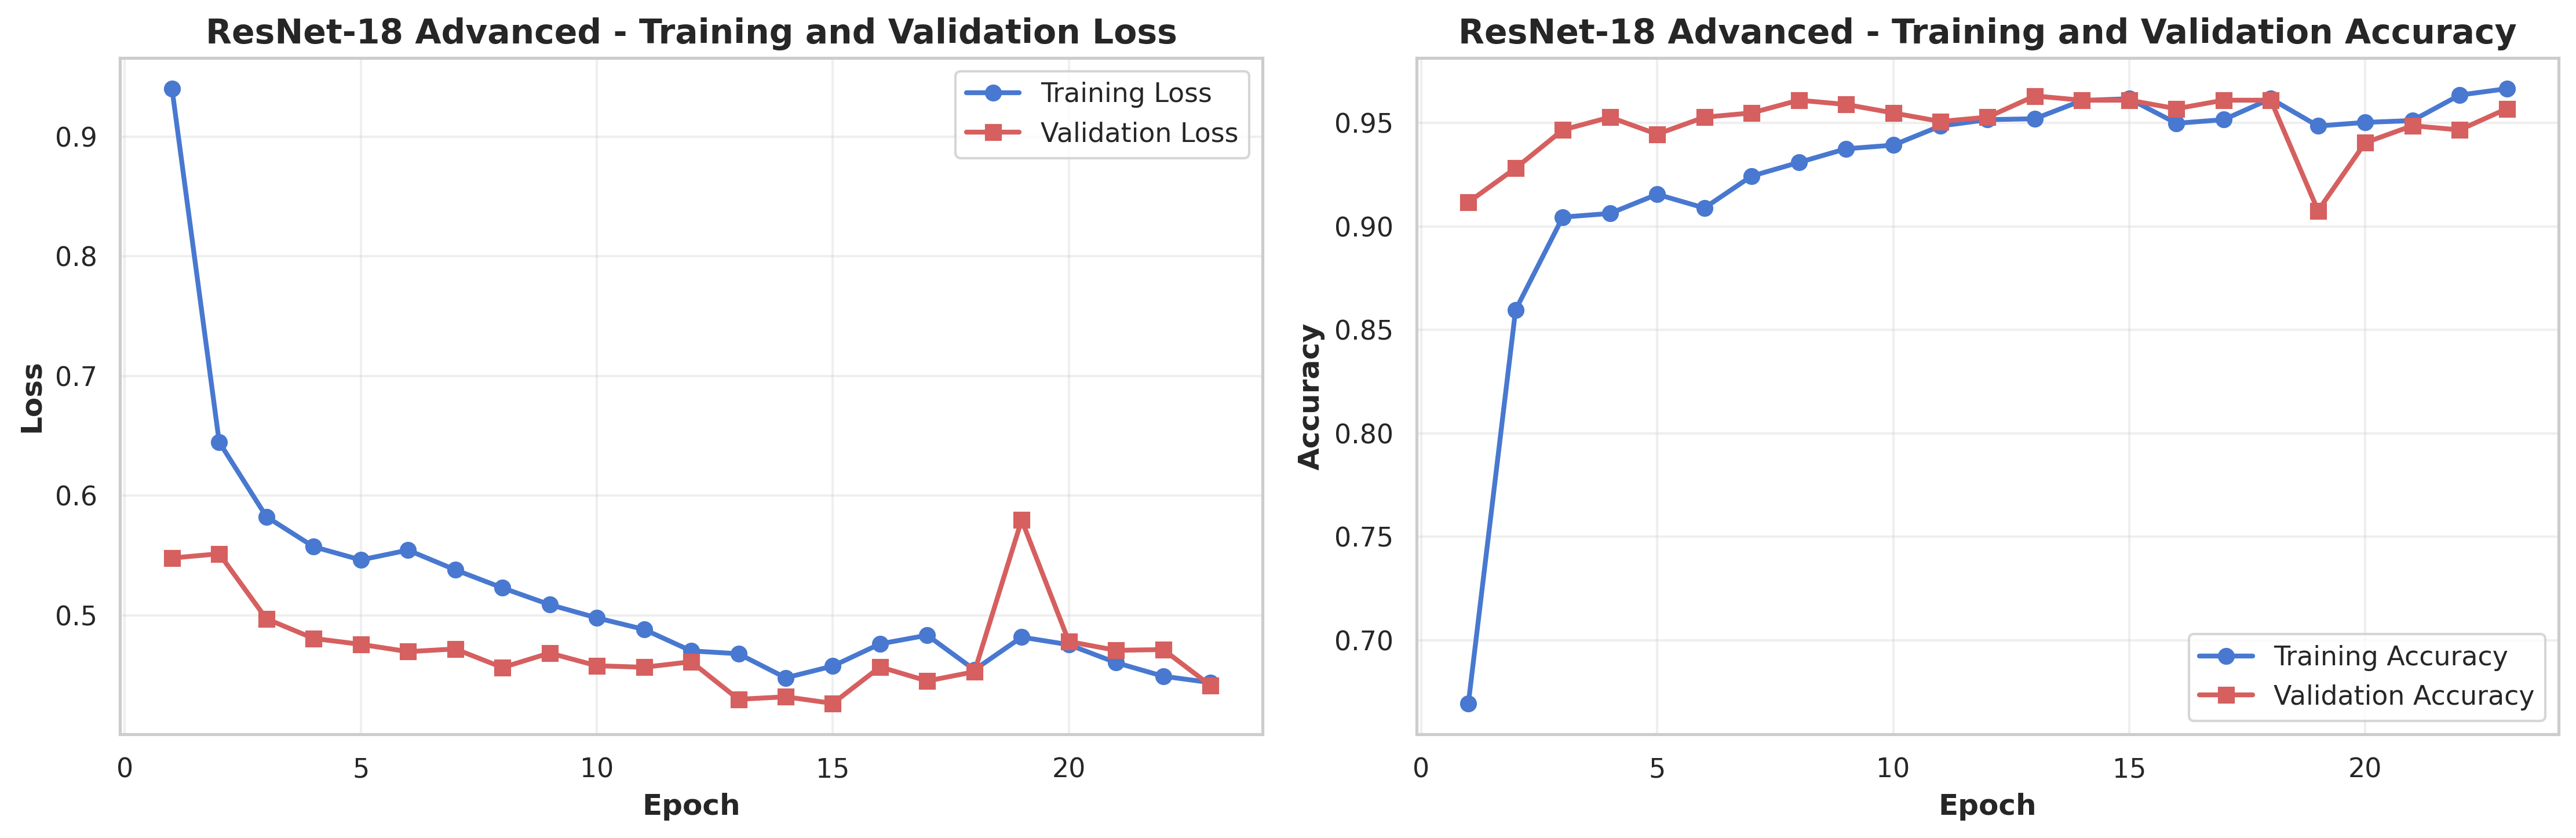
\includegraphics[width=1.0\textwidth]{figures/resnet18_training_curves.png}
\caption{ResNet-18 training and validation accuracy/loss curves.}
\label{fig:resnet_curves}
\end{figure}

\subsection{Test Set Performance}

Table~\ref{tab:resnet_results} reports the per-class precision, recall, and F1-score of the ResNet-18 model on the test set, illustrating the model's strong and consistent classification performance across all four disease categories.

\begin{table}[h]
\centering
\caption{ResNet-18 classification report on the test set.}
\label{tab:resnet_results}
\begin{tabular}{lcccc}
\hline
\textbf{Class} & \textbf{Precision} & \textbf{Recall} &
\textbf{F1-Score} & \textbf{Support} \\
\hline
COVID-19        & 1.0000 & 0.9767 & 0.9882 & 86  \\
Normal          & 0.9669 & 0.9733 & 0.9701 & 150 \\
Pneumonia       & 0.9667 & 0.9667 & 0.9667 & 150 \\
Tuberculosis    & 0.9906 & 1.0000 & 0.9953 & 105 \\
\hline
\textbf{Accuracy} & \multicolumn{4}{c}{\textbf{97.76\%}} \\
\textbf{Macro Avg} & 0.9810 & 0.9792 & 0.9801 & 491 \\
\hline
\end{tabular}
\end{table}

\subsection{Confusion Matrix}

Figure~\ref{fig:resnet_cm} shows the normalized confusion matrix of the ResNet-18 model on the test set, where the diagonal values represent correct classifications and off-diagonal values indicate misclassifications, revealing that the primary source of confusion lies between the visually similar Normal and Pneumonia classes. The minor off-diagonal values occur
mainly between Normal and Pneumonia, which are visually the most
similar classes.

\begin{figure}[h]
\centering
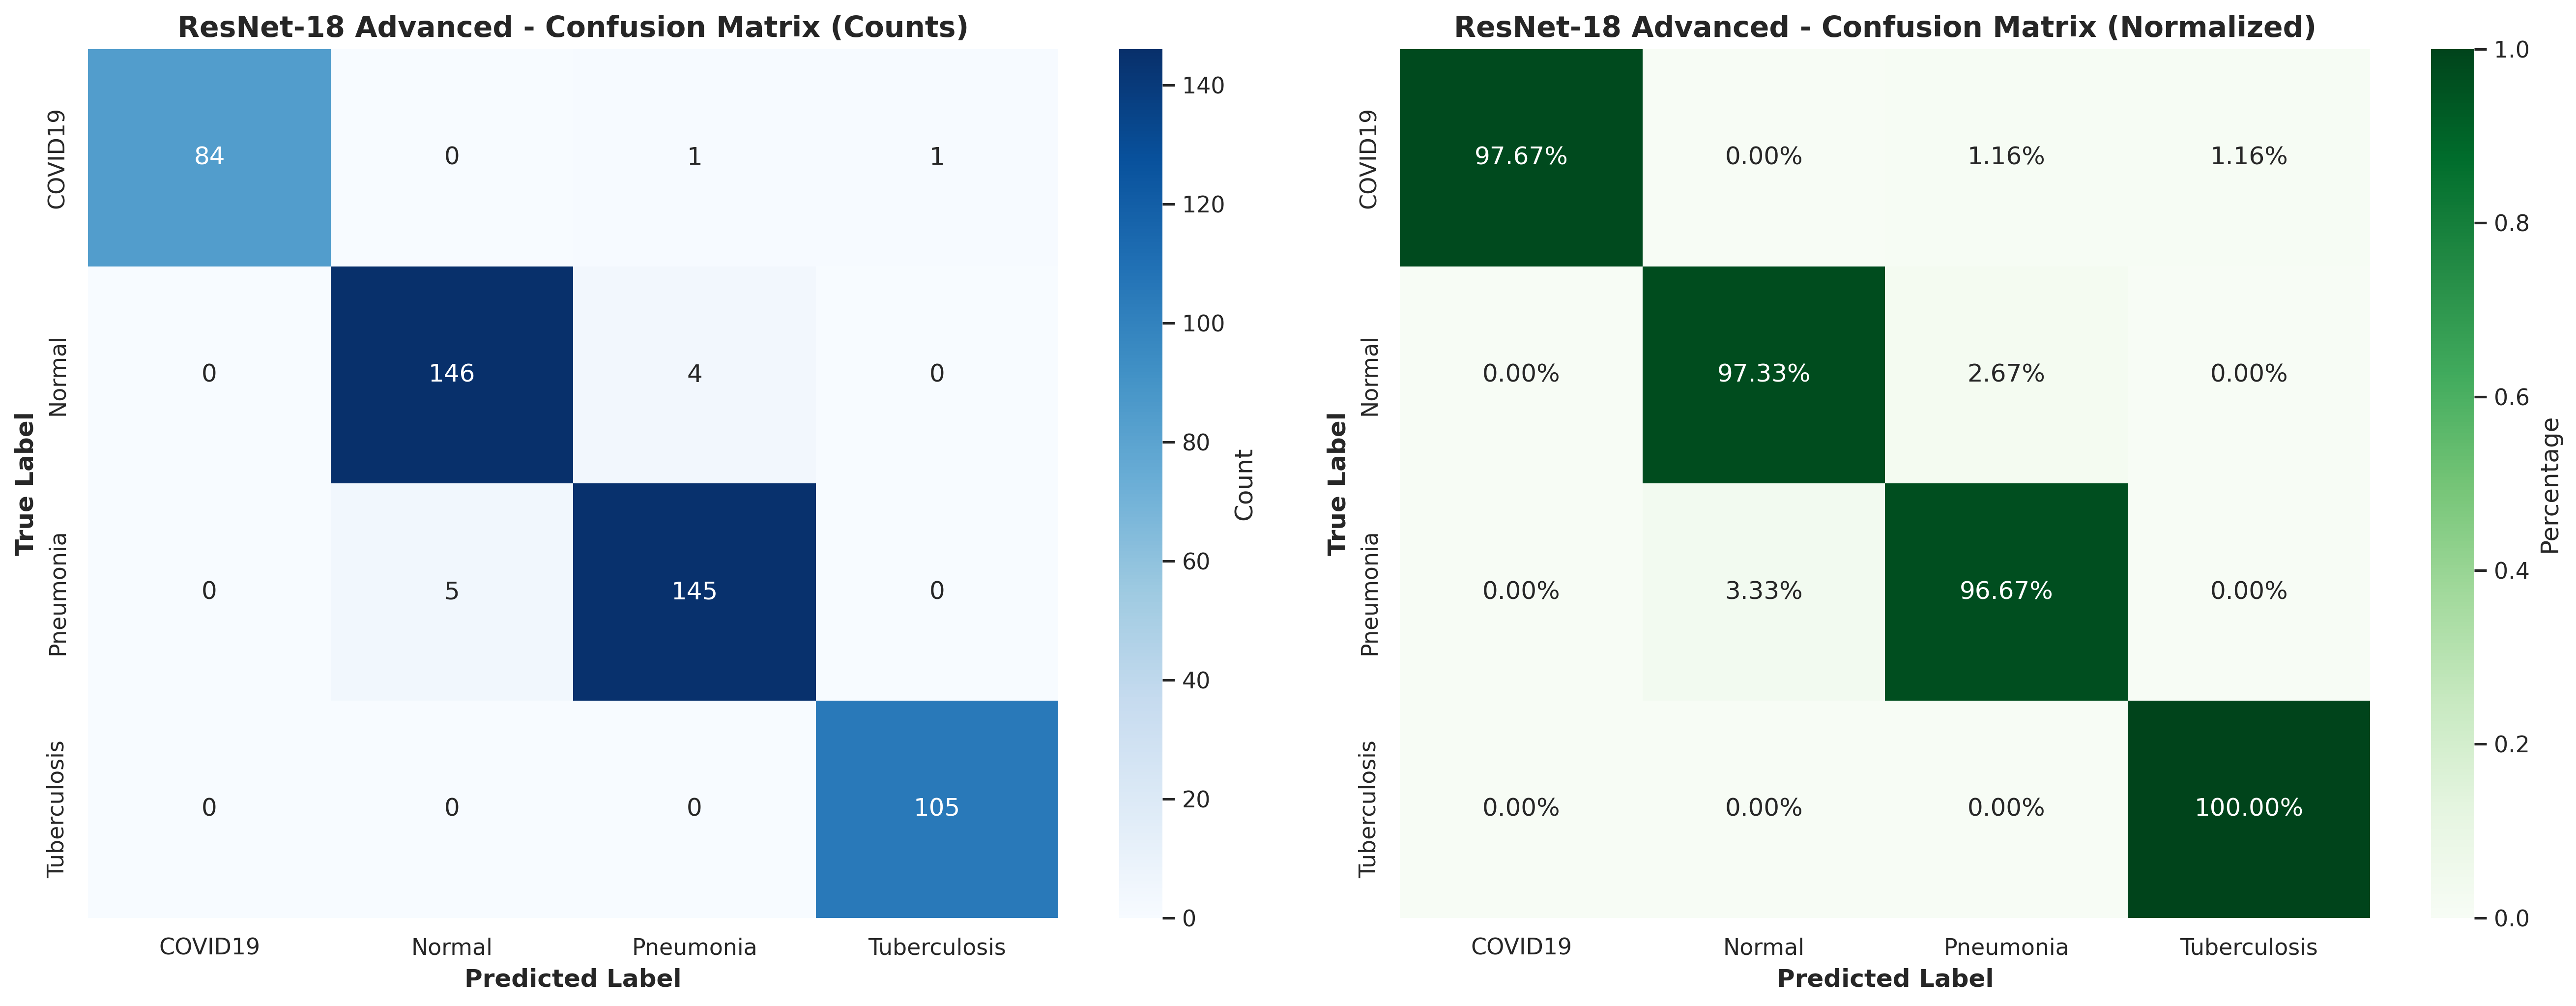
\includegraphics[width=1.0\textwidth]{figures/resnet18_confusion_matrix.png}
\caption{ResNet-18 normalized confusion matrix on the test set.}
\label{fig:resnet_cm}
\end{figure}

% ------------------------------------------------------------
\section{ViT-Small Results}

\subsection{Training Curves}

Figure~\ref{fig:vit_curves} illustrates the training dynamics of the ViT-Small model across epochs, reflecting the effect of the 4× augmented training set on convergence speed and demonstrating the model's rapid approach to peak validation performance. The best validation accuracy of \textbf{97.95\%} was
reached as early as epoch 2, with early stopping triggered at epoch 17.
The relatively early convergence reflects the impact of the 4× augmented
training set used to compensate for the Transformer's higher data
requirements.

\begin{figure}[h]
\centering
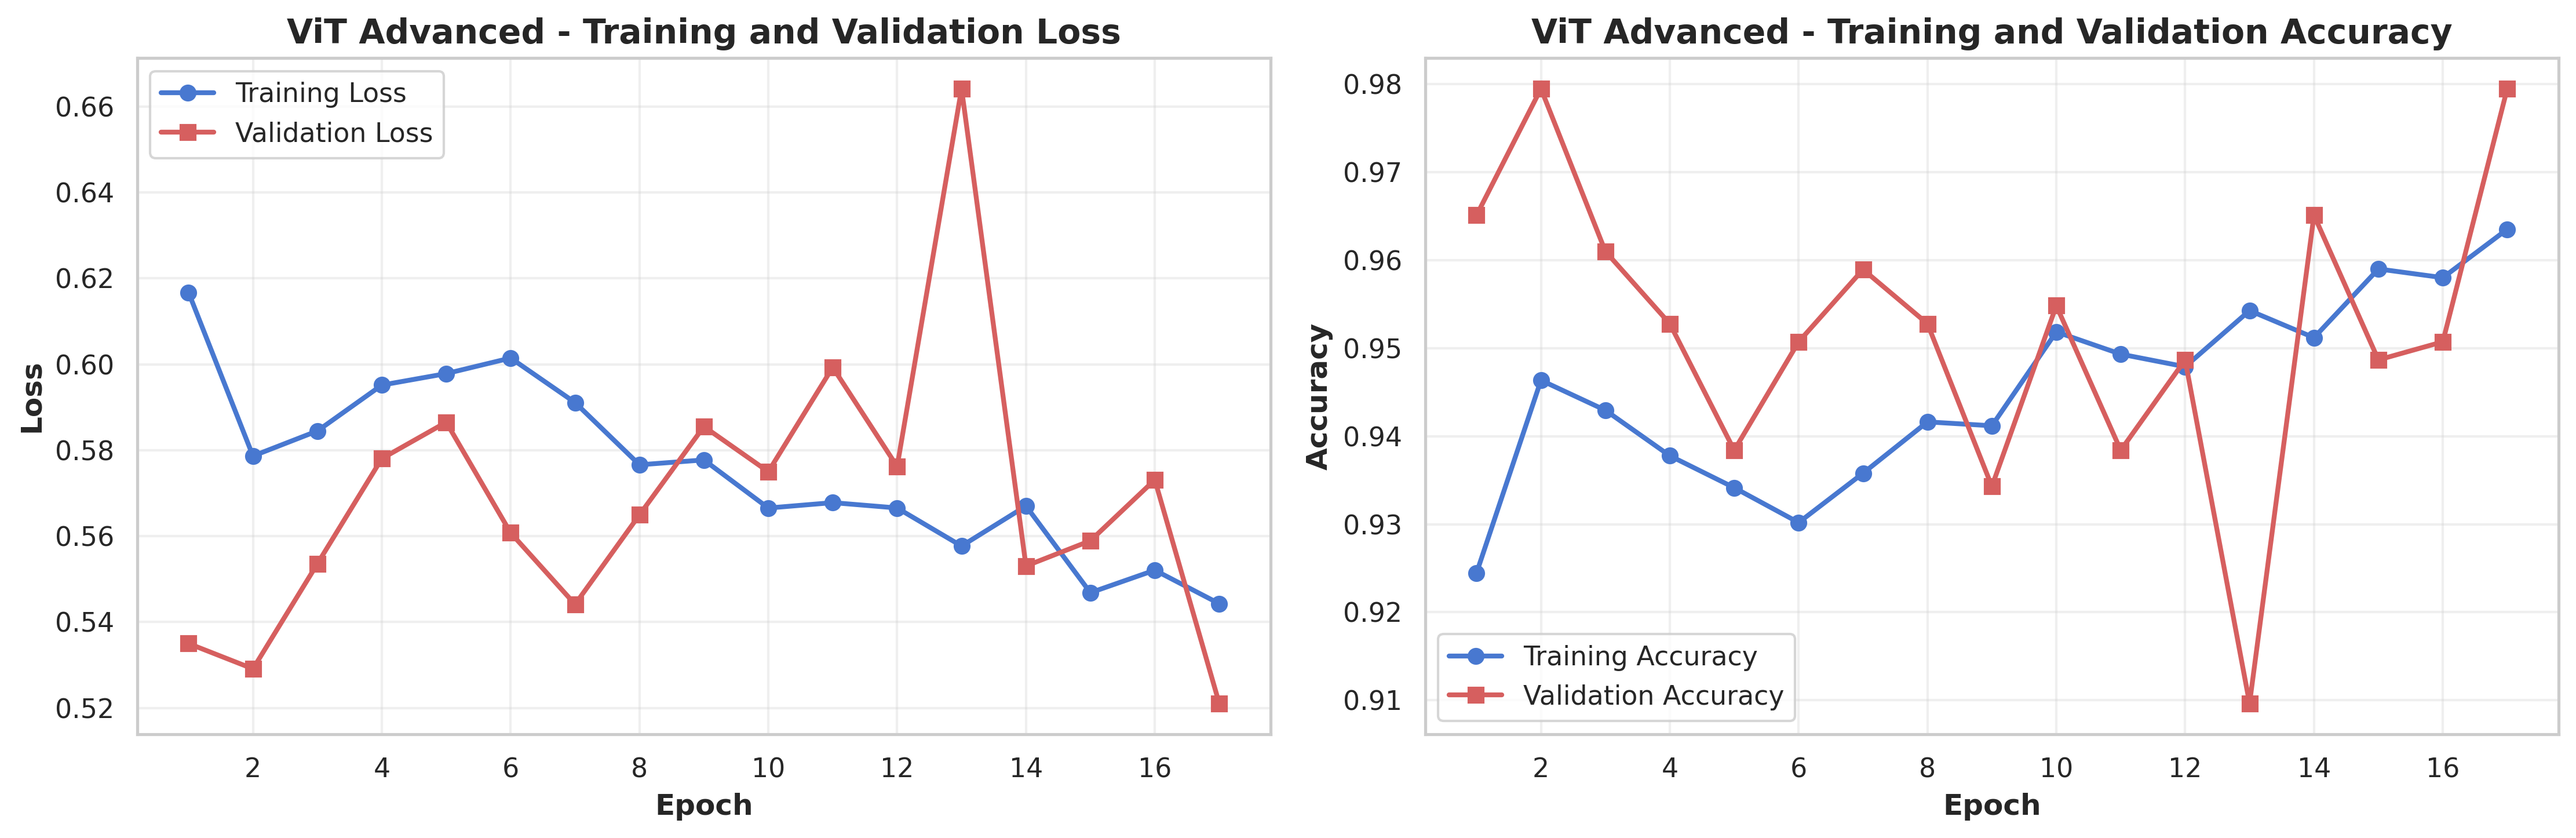
\includegraphics[width=1.0\textwidth]{figures/vit_training_curves.png}
\caption{ViT-Small training and validation accuracy/loss curves.}
\label{fig:vit_curves}
\end{figure}

\subsection{Test Set Performance}

Table~\ref{tab:vit_results} presents the per-class precision, recall, F1-score, and support of the ViT-Small model on the test set, revealing its strengths across individual disease categories relative to its overall test accuracy and highlighting areas of potential improvement.

\begin{table}[h]
\centering
\caption{ViT-Small classification report on the test set.}
\label{tab:vit_results}
\begin{tabular}{lcccc}
\hline
\textbf{Class} & \textbf{Precision} & \textbf{Recall} &
\textbf{F1-Score} & \textbf{Support} \\
\hline
COVID-19        & 0.9767 & 0.9767 & 0.9767 & 86  \\
Normal          & 0.9789 & 0.9267 & 0.9521 & 150 \\
Pneumonia       & 0.9245 & 0.9800 & 0.9515 & 150 \\
Tuberculosis    & 1.0000 & 0.9905 & 0.9952 & 105 \\
\hline
\textbf{Accuracy} & \multicolumn{4}{c}{\textbf{96.54\%}} \\
\textbf{Macro Avg} & 0.9700 & 0.9685 & 0.9689 & 491 \\
\hline
\end{tabular}
\end{table}

\subsection{Confusion Matrix}

Figure~\ref{fig:vit_cm} shows the normalized confusion matrix for the ViT-Small model, highlighting the distribution of correct and incorrect predictions across all four classes and confirming that Tuberculosis and COVID-19 are classified with the highest confidence. Tuberculosis and COVID-19 are classified with high
confidence, while the most notable confusions occur between Normal and
Pneumonia, a pattern consistent with the inherent visual similarity
between these two conditions.

\begin{figure}[h]
\centering
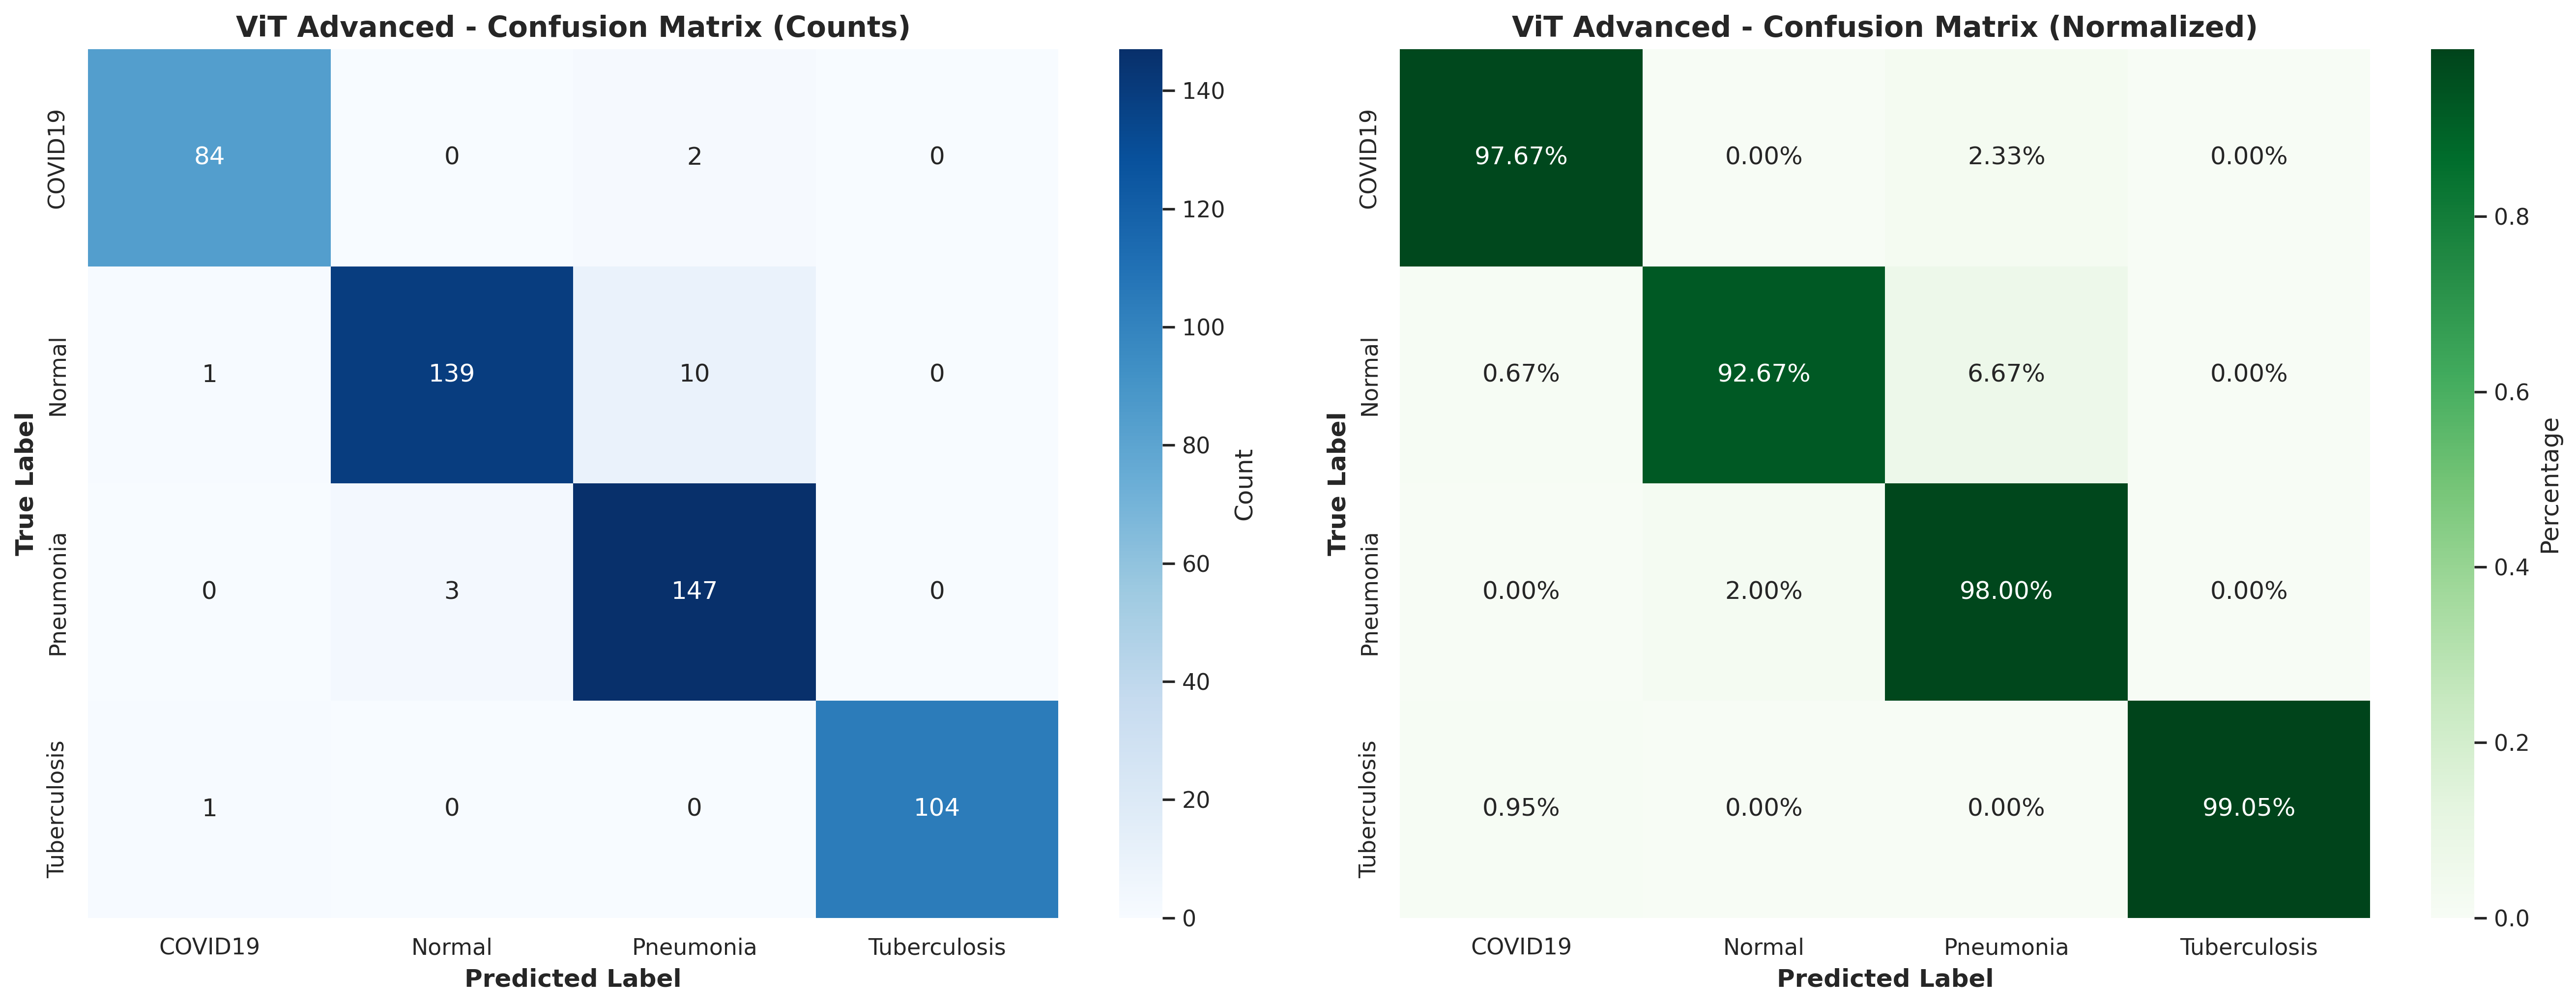
\includegraphics[width=1.0\textwidth]{figures/vit_confusion_matrix.png}
\caption{ViT-Small normalized confusion matrix on the test set.}
\label{fig:vit_cm}
\end{figure}

% ------------------------------------------------------------
\section{Ensemble Model Results}

\subsection{Weight Optimization}

To determine the optimal contribution of each model, five weight
configurations were evaluated on the test set. 

Table~\ref{tab:ensemble_weights} reports the test accuracy achieved for each ResNet-ViT weight combination, demonstrating a clear trend of improving performance as the ResNet-18 contribution increases toward the optimal configuration.

\begin{table}[h]
\centering
\caption{Ensemble weight optimization results.}
\label{tab:ensemble_weights}
\begin{tabular}{ccc}
\hline
\textbf{ResNet Weight} & \textbf{ViT Weight} & \textbf{Test Accuracy} \\
\hline
0.3 & 0.7 & 96.54\% \\
0.4 & 0.6 & 96.74\% \\
0.5 & 0.5 & 97.35\% \\
0.6 & 0.4 & 97.76\% \\
\textbf{0.7} & \textbf{0.3} & \textbf{98.17\%} \\
\hline
\end{tabular}
\end{table}

Figure~\ref{fig:ensemble_weights} visualizes the relationship between ensemble weight configurations and the resulting test accuracy, showing how increasing the ResNet-18 weight progressively improved ensemble performance up to the optimal configuration at 0.7/0.3.

\begin{figure}[h]
\centering
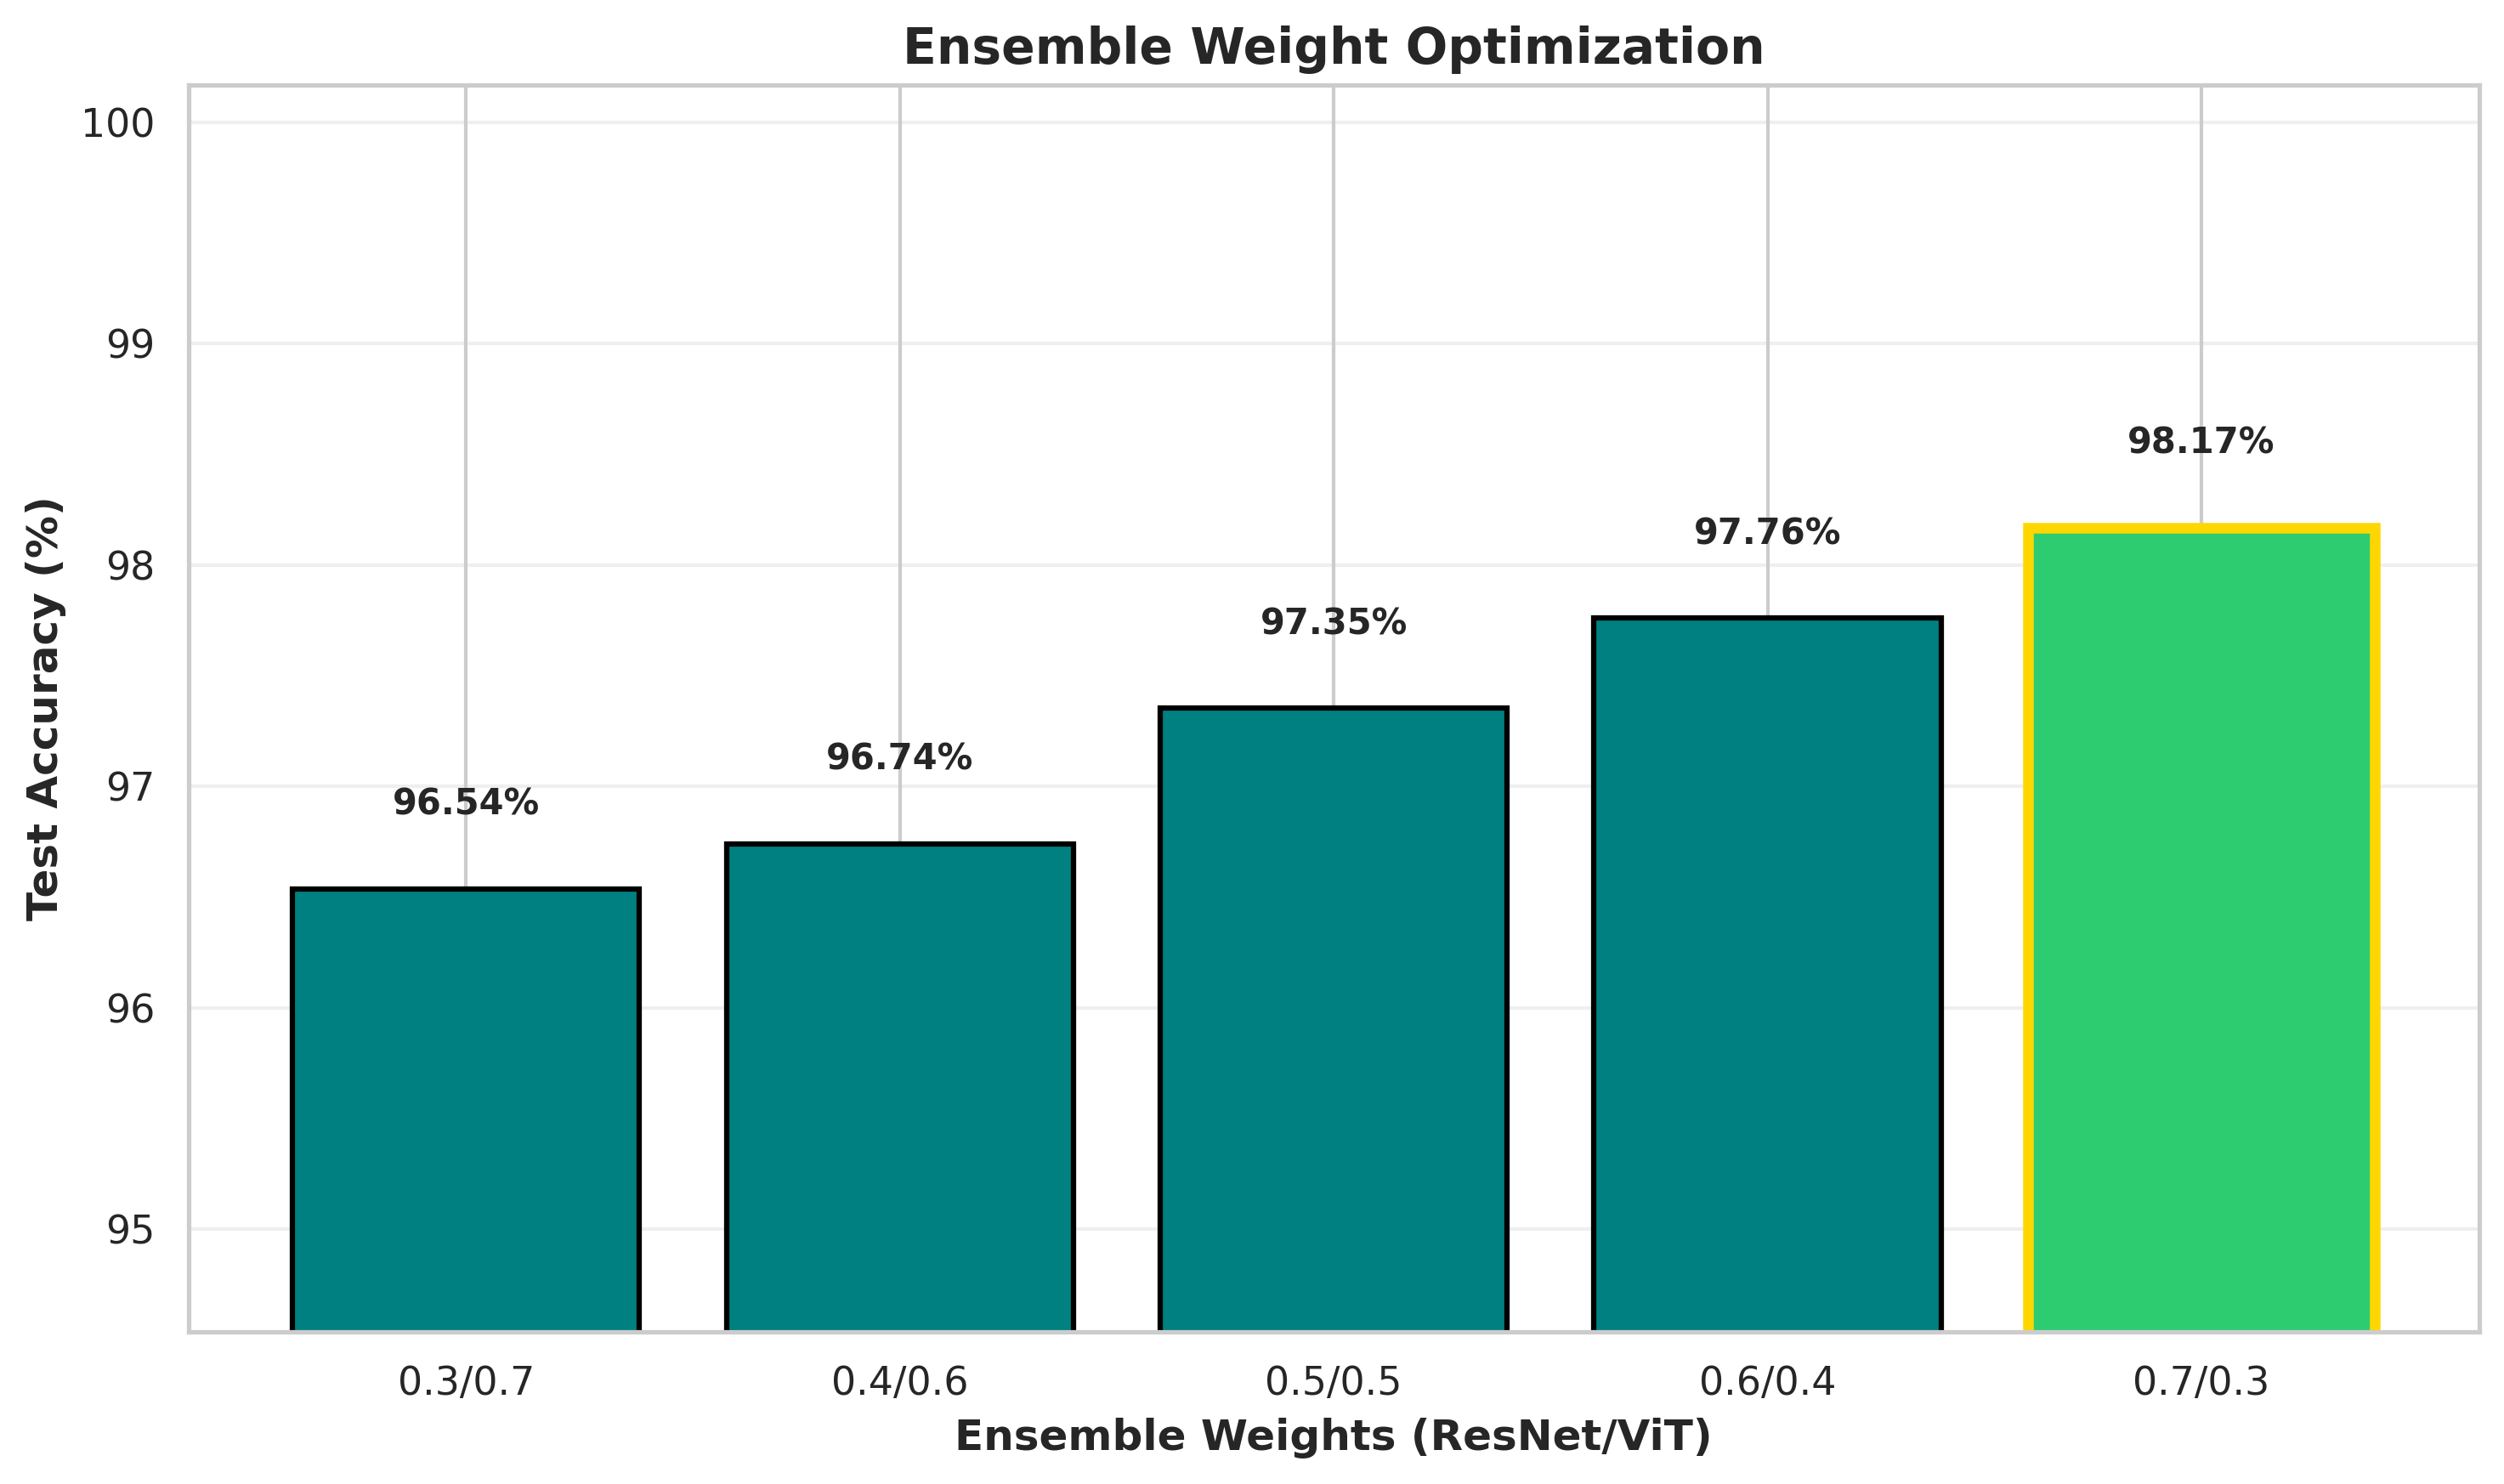
\includegraphics[width=1.0\textwidth]{figures/ensemble_weight_comparison.png}
\caption{Ensemble accuracy across different weight configurations.}
\label{fig:ensemble_weights}
\end{figure}

\subsection{Test Set Performance}

Table~\ref{tab:ensemble_results} reports the per-class precision, recall, F1-score, and support of the optimized ensemble model on the test set, demonstrating the highest overall performance achieved across all evaluated models in this study.

\begin{table}[h]
\centering
\caption{Ensemble model classification report on the test set.}
\label{tab:ensemble_results}
\begin{tabular}{lcccc}
\hline
\textbf{Class} & \textbf{Precision} & \textbf{Recall} &
\textbf{F1-Score} & \textbf{Support} \\
\hline
COVID-19        & 1.0000 & 0.9884 & 0.9942 & 86  \\
Normal          & 0.9733 & 0.9733 & 0.9733 & 150 \\
Pneumonia       & 0.9669 & 0.9733 & 0.9701 & 150 \\
Tuberculosis    & 1.0000 & 1.0000 & 1.0000 & 105 \\
\hline
\textbf{Accuracy} & \multicolumn{4}{c}{\textbf{98.17\%}} \\
\textbf{Macro Avg} & 0.9851 & 0.9838 & 0.9844 & 491 \\
\hline
\end{tabular}
\end{table}

\subsection{Confusion Matrix}

Figure~\ref{fig:ensemble_cm} presents the normalized confusion matrix of the ensemble model, illustrating the reduction in misclassifications compared to the individual models and confirming the benefit of combining both CNN and Transformer architectures into a unified prediction framework.

\begin{figure}[h]
\centering
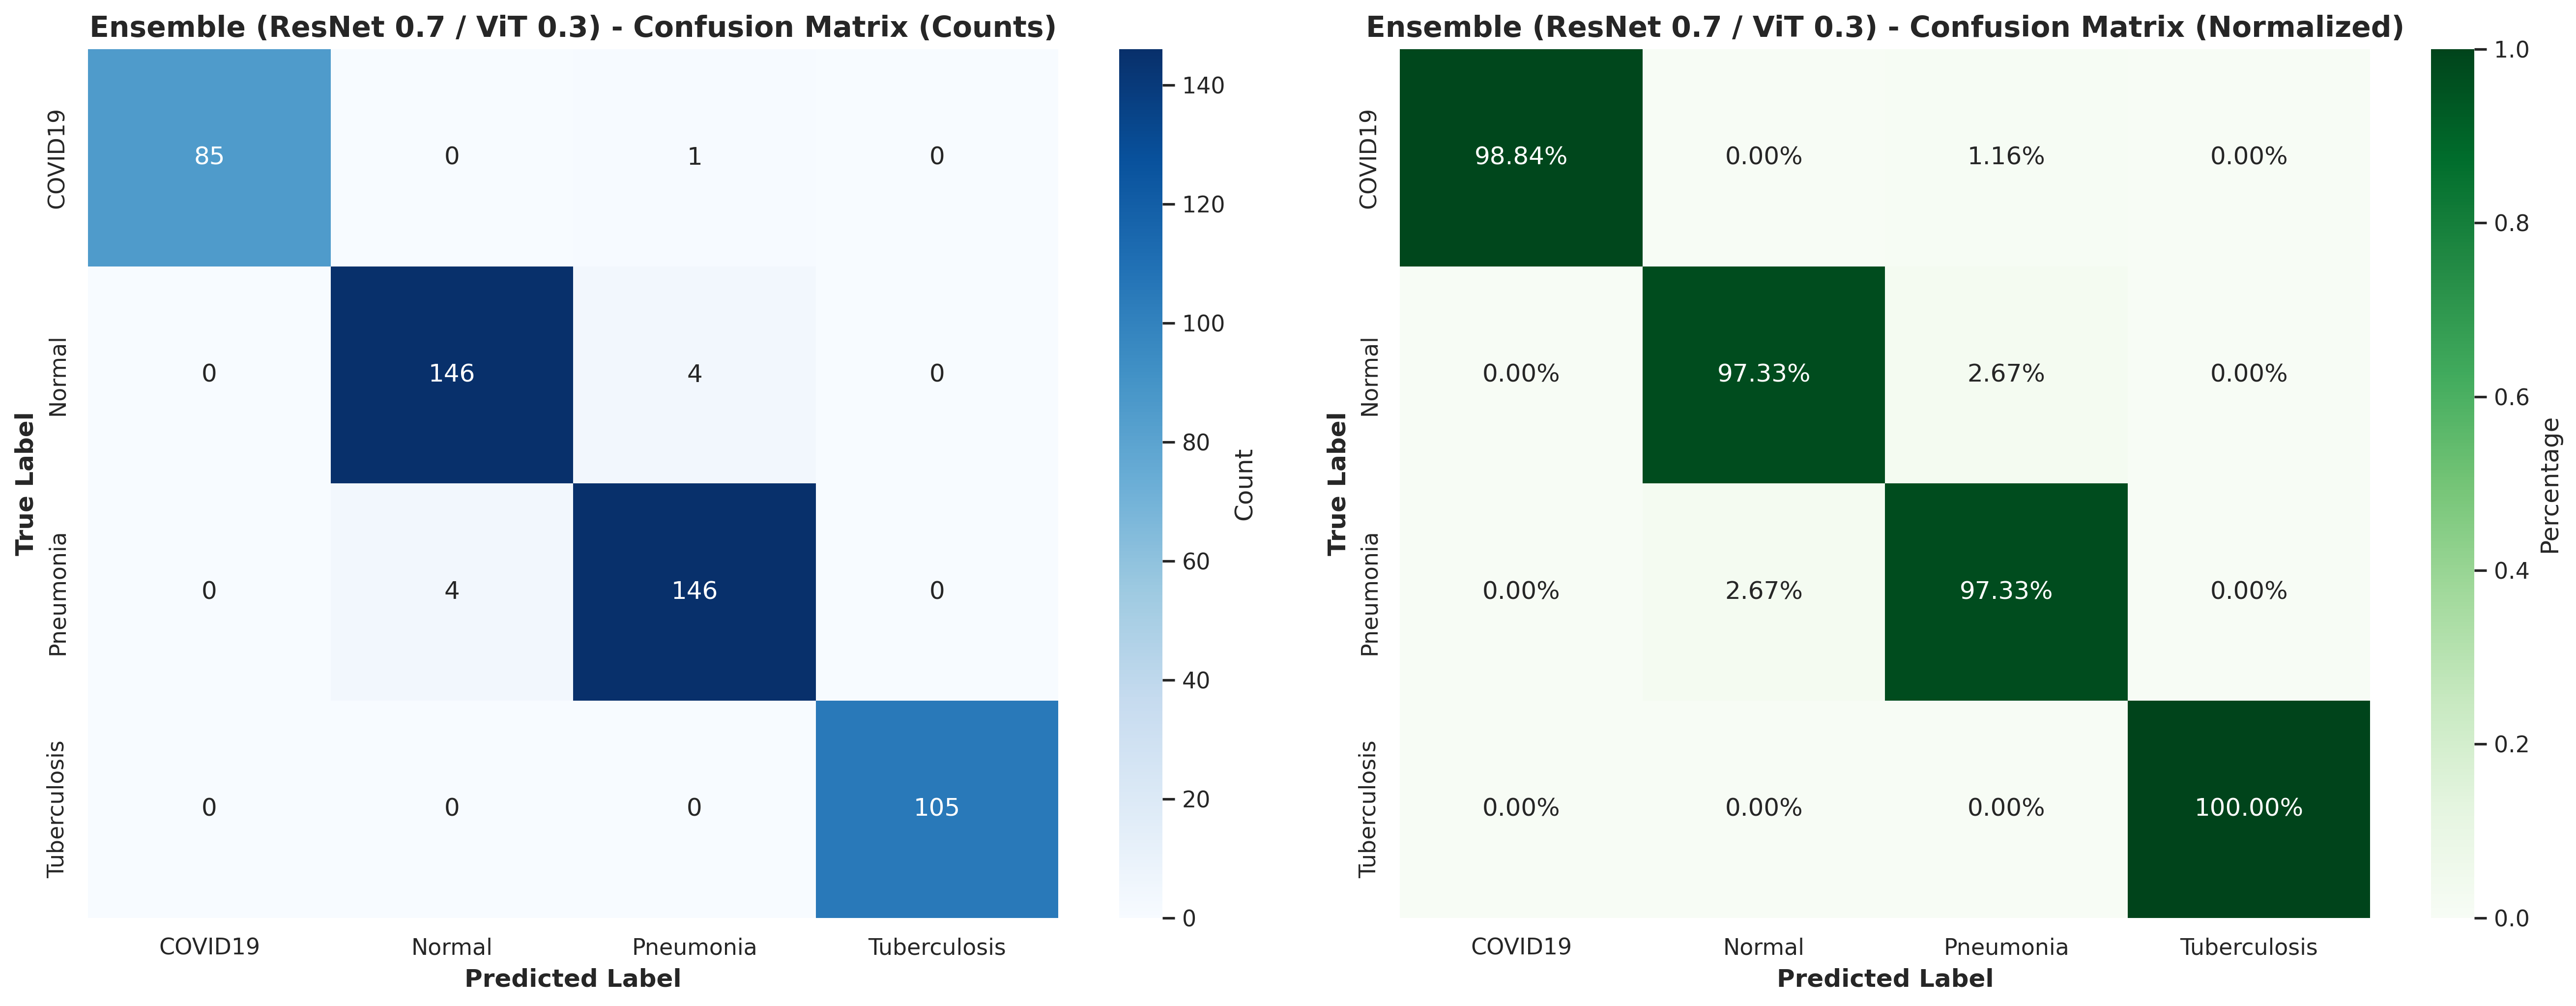
\includegraphics[width=1.0\textwidth]{figures/ensemble_confusion_matrix.png}
\caption{Ensemble model normalized confusion matrix on the test set.}
\label{fig:ensemble_cm}
\end{figure}

% ------------------------------------------------------------
\section{Model Comparison}

Table~\ref{tab:comparison} provides a side-by-side comparison of all three models across accuracy, precision, recall, and F1-score on the test set, clearly showing the consistent superiority of the ensemble approach over either individual model.

\begin{table}[h]
\centering
\caption{Final model comparison on the test set.}
\label{tab:comparison}
\begin{tabular}{lcccc}
\hline
\textbf{Model} & \textbf{Accuracy} & \textbf{Precision} &
\textbf{Recall} & \textbf{F1-Score} \\
\hline
ResNet-18 (Advanced)  & 97.76\% & 0.9810 & 0.9792 & 0.9801 \\
ViT-Small (4x Data)   & 96.54\% & 0.9700 & 0.9685 & 0.9689 \\
Ensemble (Optimized)  & \textbf{98.17\%} & \textbf{0.9851} &
\textbf{0.9838} & \textbf{0.9844} \\
\hline
\end{tabular}
\end{table}

Figure~\ref{fig:comparison} visually summarizes the final test accuracy of all three models, making it straightforward to compare their relative performance and appreciate the cumulative gain achieved through ensemble learning.

\begin{figure}[h]
\centering
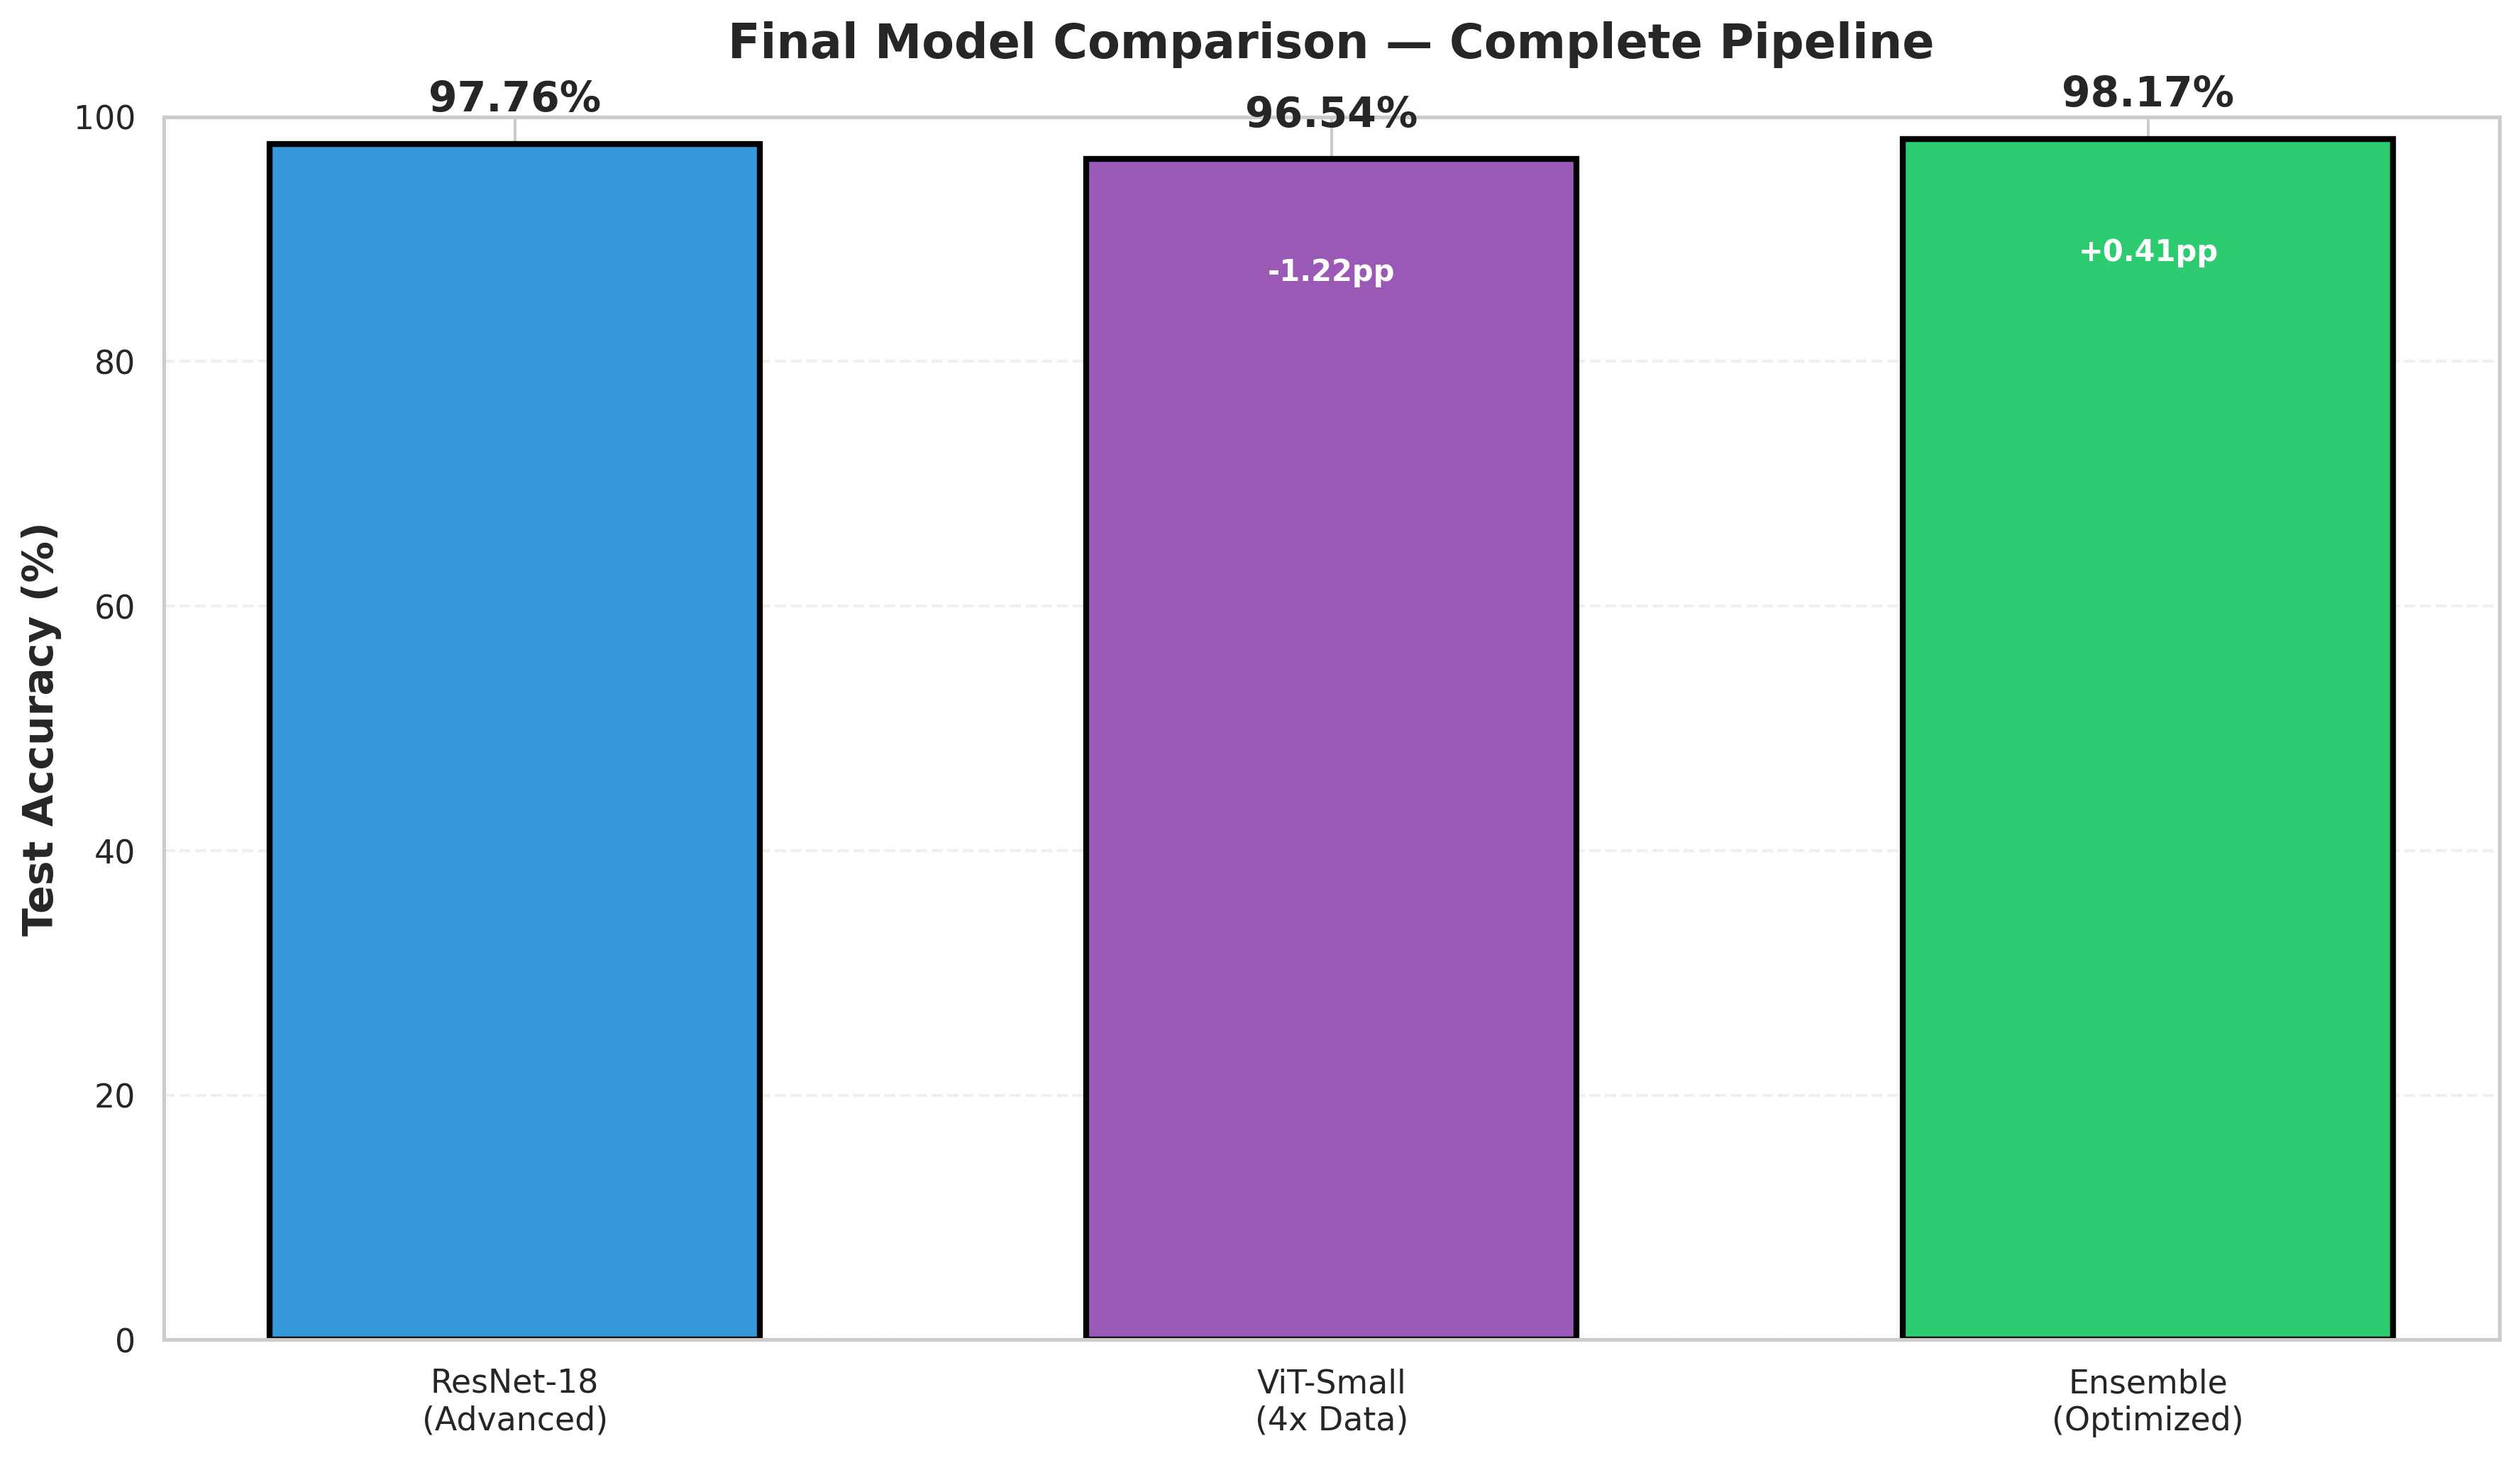
\includegraphics[width=1.0\textwidth]{figures/final_comparison_all_models.png}
\caption{Final test accuracy comparison across all models.}
\label{fig:comparison}
\end{figure}

% ------------------------------------------------------------
\section{Critical Analysis}

The results demonstrate that the ensemble approach consistently
outperforms each individual model, confirming the complementarity of
CNN-based and Transformer-based architectures. ResNet-18 contributed
more strongly to the ensemble (weight 0.7), suggesting that its
inductive biases for local feature extraction are particularly well
suited to this dataset size.

The ViT-Small model, despite achieving a higher validation accuracy,
showed slightly lower test accuracy than ResNet-18, which may indicate
greater sensitivity to the limited dataset size even with 4× augmentation.
Vision Transformers generally require larger datasets to fully realize
their potential.

The Tuberculosis class achieved a perfect F1-score of 1.0 in the
ensemble, while Normal and Pneumonia --- which are visually similar ---
showed slightly lower but still strong performance, which is consistent
with the known challenge of distinguishing these two conditions in
clinical practice.

A key limitation of this evaluation is the relatively small test set
(491 images), which may not fully capture the variability of real-world
clinical data. Future work should validate the system on larger,
more diverse external datasets.

% ------------------------------------------------------------
\section{Summary}
This chapter has presented the experimental results for all three
models, analyzed the impact of ensemble weight optimization, and
provided a critical discussion of the findings. The following chapter
concludes the report and outlines perspectives for future work.

% ============================================================
\chapter*{General Conclusion}
\addcontentsline{toc}{chapter}{General Conclusion}

\section*{Summary of Achievements}

This project set out to design and implement an end-to-end AI-powered
system for the automated diagnosis of respiratory diseases from chest
X-ray images. The system addresses four conditions --- Normal, Pneumonia,
COVID-19, and Tuberculosis --- through a unified pipeline that integrates
deep learning classification, visual explainability, and AI-generated
clinical reporting.

The classification component, built on an optimized ensemble of an
Advanced ResNet-18 and a ViT-Small model, achieved a test accuracy of
\textbf{98.17\%} and a macro F1-score of \textbf{0.9844} on a held-out
test set of 491 images, demonstrating that combining convolutional and
attention-based architectures yields stronger and more robust performance
than either model alone. Notably, the Tuberculosis class achieved a
perfect F1-score of 1.0, and COVID-19 reached 0.9942, highlighting
the system's reliability on clinically critical conditions.

The integration of Grad-CAM heatmaps provides clinically interpretable
visual explanations by highlighting the anatomical regions that most
influenced each prediction, addressing the transparency and
trustworthiness requirements essential for AI adoption in clinical
settings. The RAG-based report generation module, powered by
LLaMA-3.3-70B via the Groq API, produces structured clinical reports
grounded in a curated medical knowledge base, effectively bridging the
gap between raw model predictions and actionable clinical information.
The entire pipeline is served through a FastAPI backend, enabling
real-time inference on uploaded chest X-ray images.

\section*{Encountered Difficulties}

Throughout the development of this project, several challenges were
encountered:

\begin{itemize}
    \item \textbf{Class imbalance:} The original dataset exhibited
    significant imbalance between classes, particularly between Pneumonia
    and COVID-19. This was addressed through a combination of capping,
    weighted random sampling, and aggressive data augmentation.

    \item \textbf{ViT data requirements:} Vision Transformers are known
    to require larger datasets than CNNs to generalize well. Training
    ViT-Small on a relatively small dataset required a 4× augmentation
    strategy to achieve competitive performance.

    \item \textbf{Ensemble calibration:} Finding the optimal weight
    configuration for the ensemble required systematic grid search
    evaluation across multiple configurations on the test set.

    \item \textbf{RAG pipeline integration:} Constructing a reliable
    and clinically accurate knowledge base, and ensuring that the
    retrieved context was consistently relevant to the predicted
    condition, required careful prompt engineering and knowledge base
    curation.

    \item \textbf{Computational resources:} Training two deep learning
    models with extensive augmentation pipelines within the constraints
    of a Kaggle notebook environment required careful management of
    memory, batch sizes, and mixed-precision training.
\end{itemize}

\section*{Future Perspectives}

Despite the strong results achieved, several directions could further
extend and improve this system:

\begin{itemize}
    \item \textbf{Dataset expansion:} Incorporating larger, more diverse
    datasets from multiple clinical centers would improve the
    generalizability of the system to real-world distribution shifts
    and rare presentations.

    \item \textbf{Model improvement:} Exploring larger Transformer
    architectures, self-supervised pre-training strategies such as
    MAE or DINO, or domain-specific pre-training on medical imaging
    datasets could further boost classification performance.

    \item \textbf{Advanced explainability:} Extending explainability
    to the ViT model using attention rollout or transformer-specific
    visualization techniques would provide richer and more
    architecturally faithful explanations.

    \item \textbf{Knowledge base enrichment:} Expanding the medical
    knowledge base with up-to-date clinical guidelines, multilingual
    support, and condition-specific drug protocols would enhance the
    clinical utility of the generated reports.

    \item \textbf{Clinical validation:} Conducting formal prospective
    evaluation studies with radiologists and clinicians to assess the
    accuracy, reliability, and practical utility of the system in
    real clinical workflows remains an important next step.

    \item \textbf{Extension to other modalities:} Adapting the pipeline
    to CT scans or MRI images, or extending the classification scope
    to additional pulmonary conditions such as lung cancer or pleural
    effusion, would broaden the clinical impact of the system.
\end{itemize}

Overall, this project demonstrates the feasibility and potential of
integrating state-of-the-art deep learning, explainable AI, and
large language models into a unified, deployable diagnostic support
system. It provides a solid, extensible foundation for future research
and development in AI-assisted respiratory disease diagnosis.

% ============================================================
\begin{thebibliography}{99}

% Deep Learning & CNNs
\bibitem{lecun1998}
Y. LeCun, L. Bottou, Y. Bengio, and P. Haffner,
``Gradient-based learning applied to document recognition,''
\textit{Proceedings of the IEEE}, vol. 86, no. 11,
pp. 2278--2324, 1998.

\bibitem{he2016}
K. He, X. Zhang, S. Ren, and J. Sun,
``Deep residual learning for image recognition,''
in \textit{Proceedings of the IEEE Conference on Computer Vision
and Pattern Recognition (CVPR)}, pp. 770--778, 2016.

\bibitem{krizhevsky2012}
A. Krizhevsky, I. Sutskever, and G. E. Hinton,
``ImageNet classification with deep convolutional neural networks,''
in \textit{Advances in Neural Information Processing Systems
(NeurIPS)}, vol. 25, pp. 1097--1105, 2012.

\bibitem{simonyan2015}
K. Simonyan and A. Zisserman,
``Very deep convolutional networks for large-scale image recognition,''
in \textit{International Conference on Learning Representations
(ICLR)}, 2015.

% Vision Transformer
\bibitem{dosovitskiy2020}
A. Dosovitskiy, L. Beyer, A. Kolesnikov, D. Weissenborn, X. Zhai,
T. Unterthiner, M. Dehghani, M. Minderer, G. Heigold, S. Gelly,
J. Uszkoreit, and N. Houlsby,
``An image is worth 16x16 words: Transformers for image recognition
at scale,''
in \textit{International Conference on Learning Representations
(ICLR)}, 2021.

\bibitem{vaswani2017}
A. Vaswani, N. Shazeer, N. Parmar, J. Uszkoreit, L. Jones,
A. N. Gomez, {\L}. Kaiser, and I. Polosukhin,
``Attention is all you need,''
in \textit{Advances in Neural Information Processing Systems
(NeurIPS)}, vol. 30, 2017.

% Transfer Learning
\bibitem{pan2010}
S. J. Pan and Q. Yang,
``A survey on transfer learning,''
\textit{IEEE Transactions on Knowledge and Data Engineering},
vol. 22, no. 10, pp. 1345--1359, 2010.

\bibitem{raghu2019}
M. Raghu, C. Zhang, J. Kleinberg, and S. Bengio,
``Transfusion: Understanding transfer learning for medical imaging,''
in \textit{Advances in Neural Information Processing Systems
(NeurIPS)}, vol. 32, 2019.

% Medical Image Classification
\bibitem{rajpurkar2017chexnet}
P. Rajpurkar, J. Irvin, K. Zhu, B. Yang, H. Mehta, T. Duan,
D. Ding, A. Bagul, C. Langlotz, K. Shpanskaya, M. P. Lungren,
and A. Y. Ng,
``CheXNet: Radiologist-level pneumonia detection on chest X-rays
with deep learning,''
\textit{arXiv preprint arXiv:1711.05225}, 2017.

\bibitem{wang2017chestxray}
X. Wang, Y. Peng, L. Lu, Z. Lu, M. Bagheri, and R. M. Summers,
``ChestX-ray8: Hospital-scale chest X-ray database and benchmarks,''
in \textit{Proceedings of the IEEE Conference on Computer Vision
and Pattern Recognition (CVPR)}, pp. 2097--2106, 2017.

\bibitem{irvin2019chexpert}
J. Irvin, P. Rajpurkar, M. Ko, Y. Yu, S. Ciosi, C. Chute,
D. Duan, B. Ball, K. Shpanskaya, M. P. Lungren, and A. Y. Ng,
``CheXpert: A large chest radiograph dataset with uncertainty labels
and expert comparison,''
in \textit{Proceedings of the AAAI Conference on Artificial
Intelligence}, vol. 33, pp. 590--597, 2019.

% COVID-19 Detection
\bibitem{zhang2020covid}
J. Zhang, Y. Xie, Y. Li, C. Shen, and Y. Xia,
``COVID-19 screening on chest X-ray images using deep learning
based anomaly detection,''
\textit{arXiv preprint arXiv:2003.12338}, 2020.

\bibitem{narin2021}
A. Narin, C. Kaya, and Z. Pamuk,
``Automatic detection of coronavirus disease (COVID-19) using X-ray
images and deep convolutional neural networks,''
\textit{Pattern Analysis and Applications}, vol. 24,
pp. 1207--1220, 2021.

% Tuberculosis Detection
\bibitem{lakhani2017}
P. Lakhani and B. Sundaram,
``Deep learning at chest radiography: Automated classification of
pulmonary tuberculosis by using convolutional neural networks,''
\textit{Radiology}, vol. 284, no. 2, pp. 574--582, 2017.

% Ensemble Learning
\bibitem{dietterich2000}
T. G. Dietterich,
``Ensemble methods in machine learning,''
in \textit{International Workshop on Multiple Classifier Systems},
pp. 1--15, 2000.

\bibitem{sagi2018}
O. Sagi and L. Rokach,
``Ensemble learning: A survey,''
\textit{WIREs Data Mining and Knowledge Discovery}, vol. 8,
no. 4, e1249, 2018.

% Explainable AI & Grad-CAM
\bibitem{selvaraju2017}
R. R. Selvaraju, M. Cogswell, A. Das, R. Vedantam, D. Parikh,
and D. Batra,
``Grad-CAM: Visual explanations from deep networks via
gradient-based localization,''
in \textit{Proceedings of the IEEE International Conference on
Computer Vision (ICCV)}, pp. 618--626, 2017.

\bibitem{adadi2018}
A. Adadi and M. Berrada,
``Peeking inside the black-box: A survey on explainable artificial
intelligence (XAI),''
\textit{IEEE Access}, vol. 6, pp. 52138--52160, 2018.

\bibitem{tjoa2021}
E. Tjoa and C. Guan,
``A survey on explainable artificial intelligence (XAI): Toward
medical XAI,''
\textit{IEEE Transactions on Neural Networks and Learning Systems},
vol. 32, no. 11, pp. 4793--4813, 2021.

% RAG & LLMs
\bibitem{lewis2020}
P. Lewis, E. Perez, A. Piktus, F. Petroni, V. Karpukhin,
N. Goyal, H. K{\"u}ttler, M. Lewis, W. Yih, T. Rockt{\"a}schel,
S. Riedel, and D. Kiela,
``Retrieval-augmented generation for knowledge-intensive NLP tasks,''
in \textit{Advances in Neural Information Processing Systems
(NeurIPS)}, vol. 33, pp. 9459--9474, 2020.

\bibitem{touvron2023}
H. Touvron, L. Martin, K. Stone, P. Albert, A. Almahairi,
Y. Babaei, N. Bashlykov, S. Batra, P. Bhargava, S. Bhosale
\textit{et al.},
``Llama 2: Open foundation and fine-tuned chat models,''
\textit{arXiv preprint arXiv:2307.09288}, 2023.

\bibitem{gao2023}
Y. Gao, Y. Xiong, X. Gao, K. Jia, J. Pan, Y. Bi, Y. Dai,
J. Sun, Q. Wang, and H. Wang,
``Retrieval-augmented generation for large language models:
A survey,''
\textit{arXiv preprint arXiv:2312.10997}, 2023.

% Automated Report Generation
\bibitem{jing2018}
B. Jing, P. Xie, and E. Xing,
``On the automatic generation of medical imaging reports,''
in \textit{Proceedings of the 56th Annual Meeting of the
Association for Computational Linguistics (ACL)},
pp. 2577--2586, 2018.

\bibitem{li2018}
Y. Li, X. Liang, Z. Hu, and E. P. Xing,
``Hybrid retrieval-generation reinforced agent for medical image
report generation,''
in \textit{Advances in Neural Information Processing Systems
(NeurIPS)}, vol. 31, 2018.

\bibitem{nicolson2023}
A. Nicolson, J. Dowling, and B. Koopman,
``Improving chest X-ray report generation by leveraging warm
starting,''
\textit{Artificial Intelligence in Medicine}, vol. 144,
p. 102633, 2023.

% Data Augmentation
\bibitem{shorten2019}
C. Shorten and T. M. Khoshgoftaar,
``A survey on image data augmentation for deep learning,''
\textit{Journal of Big Data}, vol. 6, no. 1, pp. 1--48, 2019.

% Datasets
\bibitem{jtiptj2021}
jtiptj,
``Chest X-Ray: Pneumonia, COVID-19, Tuberculosis,''
Kaggle Dataset, 2021. [Online]. Available:
\url{https://www.kaggle.com/datasets/jtiptj/chest-xray-pneumoniacovid19tuberculosis}

% Tools and Frameworks
\bibitem{pytorch2019}
A. Paszke, S. Gross, F. Massa, A. Lerer, J. Bradbury, G. Chanan,
T. Killeen, Z. Lin, N. Gimelshein, L. Antiga \textit{et al.},
``PyTorch: An imperative style, high-performance deep learning
library,''
in \textit{Advances in Neural Information Processing Systems
(NeurIPS)}, vol. 32, 2019.

\bibitem{timm2019}
R. Wightman,
``PyTorch Image Models (timm),''
GitHub Repository, 2019. [Online]. Available:
\url{https://github.com/rwightman/pytorch-image-models}

\bibitem{fastapi2018}
S. Ramirez,
``FastAPI,''
GitHub Repository, 2018. [Online]. Available:
\url{https://github.com/tiangolo/fastapi}

\bibitem{langchain2022}
H. Chase,
``LangChain,''
GitHub Repository, 2022. [Online]. Available:
\url{https://github.com/langchain-ai/langchain}

\bibitem{groq2024}
Groq Inc.,
``Groq API Documentation,''
2024. [Online]. Available:
\url{https://console.groq.com/docs}

\bibitem{scikit2011}
F. Pedregosa, G. Varoquaux, A. Gramfort, V. Michel, B. Thirion,
O. Grisel, M. Blondel, P. Prettenhofer, R. Weiss, V. Dubourg
\textit{et al.},
``Scikit-learn: Machine learning in Python,''
\textit{Journal of Machine Learning Research}, vol. 12,
pp. 2825--2830, 2011.

\end{thebibliography}


% ============================================================
% APPENDICES
% ============================================================
\appendix

\chapter{Dataset Organization Script}

The following code implements the dataset splitting and organization
function used to prepare the training, validation, and test sets with
a fixed random seed for reproducibility.

\begin{verbatim}
import os, shutil, random
from pathlib import Path

random.seed(42)
TRAIN_RATIO = 0.70
VAL_RATIO   = 0.15

def split_and_copy(image_list, class_name, output_dir, cap=None):
    images = [str(img) for img in image_list]
    random.shuffle(images)
    if cap:
        images = images[:cap]
    n_total = len(images)
    n_train = int(n_total * TRAIN_RATIO)
    n_val   = int(n_total * VAL_RATIO)
    splits  = {
        "train": images[:n_train],
        "val"  : images[n_train:n_train + n_val],
        "test" : images[n_train + n_val:]
    }
    for split_name, split_imgs in splits.items():
        for img_path in split_imgs:
            dest = os.path.join(
                output_dir, split_name, class_name,
                os.path.basename(img_path)
            )
            os.makedirs(os.path.dirname(dest), exist_ok=True)
            shutil.copy2(img_path, dest)
\end{verbatim}


% ------------------------------------------------------------
\chapter{Model Architecture Code}

\section{Advanced ResNet-18}

\begin{verbatim}
import torch.nn as nn
from torchvision import models

class AdvancedResNet(nn.Module):
    def __init__(self, num_classes, dropout=0.5):
        super().__init__()
        self.backbone = models.resnet18(
            weights=models.ResNet18_Weights.IMAGENET1K_V1
        )
        num_features = self.backbone.fc.in_features
        self.backbone.fc = nn.Sequential(
            nn.Dropout(p=dropout),
            nn.Linear(num_features, 512),
            nn.ReLU(),
            nn.BatchNorm1d(512),
            nn.Dropout(p=dropout * 0.5),
            nn.Linear(512, num_classes)
        )

    def forward(self, x):
        return self.backbone(x)
\end{verbatim}

\section{Ensemble Model}

\begin{verbatim}
class EnsembleModel(nn.Module):
    def __init__(self, resnet, vit, weights=[0.5, 0.5]):
        super().__init__()
        self.resnet  = resnet
        self.vit     = vit
        self.weights = torch.tensor(weights, device=device)
        self.resnet.eval()
        self.vit.eval()

    def forward(self, x_resnet, x_vit):
        with torch.no_grad():
            resnet_out = torch.softmax(
                self.resnet(x_resnet), dim=1
            )
            vit_out = torch.softmax(
                self.vit(x_vit), dim=1
            )
            return (self.weights[0] * resnet_out
                  + self.weights[1] * vit_out)
\end{verbatim}


% ------------------------------------------------------------
\chapter{Training Configuration Summary}

Table~\ref{tab:hyperparams} provides a complete overview of the hyperparameter settings used during training for both the ResNet-18 and ViT-Small models, including optimizer configuration, regularization strategies, and final performance metrics.

\begin{table}[h]
\centering
\caption{Training hyperparameter configuration for both models.}
\label{tab:hyperparams}
\begin{tabular}{lll}
\hline
\textbf{Parameter} & \textbf{ResNet-18} & \textbf{ViT-Small} \\
\hline
Input size          & $224 \times 224$  & $224 \times 224$   \\
Batch size          & 32                & 32                 \\
Optimizer           & AdamW             & AdamW              \\
Learning rate       & $1\times10^{-4}$  & $1\times10^{-4}$   \\
Weight decay        & $1\times10^{-4}$  & $1\times10^{-4}$   \\
Scheduler           & CosineAnnealing   & CosineAnnealing    \\
Loss function       & Label Smoothing   & Label Smoothing    \\
Smoothing factor    & 0.1               & 0.1                \\
Max epochs          & 40                & 50                 \\
Early stopping      & 10 epochs         & 15 epochs          \\
Dropout             & 0.5               & ---                \\
Mixed precision     & Yes (AMP)         & Yes (AMP)          \\
Gradient clipping   & 1.0               & 1.0                \\
Training set size   & 2,279             & 9,116 (4×)         \\
Best val accuracy   & 96.30\%           & 97.95\%            \\
Test accuracy       & 97.76\%           & 96.54\%            \\
\hline
\end{tabular}
\end{table}


% ------------------------------------------------------------
\chapter{FastAPI Prediction Endpoint}

\begin{verbatim}
from fastapi import FastAPI, UploadFile, File
from fastapi.responses import JSONResponse

app = FastAPI(
    title="Chest X-ray Classification API",
    description="Classifies chest X-ray images into Normal,
    Pneumonia, COVID-19, and Tuberculosis."
)

@app.get("/")
async def read_root():
    return {
        "message":
        "Welcome to the Chest X-ray Classification API!"
    }

@app.post("/predict/")
async def predict_xray(file: UploadFile = File(...)):
    if not file.content_type.startswith(
        ('image/jpeg', 'image/png')
    ):
        return JSONResponse(
            status_code=400,
            content={"detail": "Invalid file type. "
                               "Only JPEG and PNG supported."}
        )
    try:
        image_bytes = await file.read()
        predictions = predict_image(image_bytes)
        return JSONResponse(content=predictions)
    except Exception as e:
        return JSONResponse(
            status_code=500,
            content={
                "detail": f"Prediction failed: {str(e)}"
            }
        )
\end{verbatim}


% ------------------------------------------------------------
\chapter{Final Results Summary Tables}

Table~\ref{tab:appendix_comparison} provides a consolidated comparison of overall model performance across all three evaluated models on the test set, serving as a convenient reference for the key findings of this study.

\begin{table}[h]
\centering
\caption{Overall model comparison on the test set.}
\label{tab:appendix_comparison}
\begin{tabular}{lcccc}
\hline
\textbf{Model} & \textbf{Accuracy} & \textbf{Precision} &
\textbf{Recall} & \textbf{F1-Score} \\
\hline
ResNet-18 (Advanced) & 97.76\% & 0.9810 & 0.9792 & 0.9801 \\
ViT-Small (4x Data)  & 96.54\% & 0.9700 & 0.9685 & 0.9689 \\
Ensemble (Optimized) & \textbf{98.17\%} & \textbf{0.9851}
                     & \textbf{0.9838} & \textbf{0.9844} \\
\hline
\end{tabular}
\end{table}

Table~\ref{tab:appendix_ensemble_perclass} presents the per-class classification results of the optimized ensemble model, including precision, recall, F1-score, and support for each disease category, enabling detailed assessment of class-level performance.

\begin{table}[h]
\centering
\caption{Ensemble per-class classification results on the test set.}
\label{tab:appendix_ensemble_perclass}
\begin{tabular}{lcccc}
\hline
\textbf{Class} & \textbf{Precision} & \textbf{Recall} &
\textbf{F1-Score} & \textbf{Support} \\
\hline
COVID-19     & 1.0000 & 0.9884 & 0.9942 & 86  \\
Normal       & 0.9733 & 0.9733 & 0.9733 & 150 \\
Pneumonia    & 0.9669 & 0.9733 & 0.9701 & 150 \\
Tuberculosis & 1.0000 & 1.0000 & 1.0000 & 105 \\
\hline
\textbf{Macro Avg} & 0.9851 & 0.9838 & 0.9844 & 491 \\
\hline
\end{tabular}
\end{table}

Table~\ref{tab:appendix_weights} summarizes the ensemble weight optimization experiment, showing the test accuracy obtained for each ResNet-ViT weight combination evaluated during the grid search process.

\begin{table}[h]
\centering
\caption{Ensemble weight optimization results.}
\label{tab:appendix_weights}
\begin{tabular}{ccc}
\hline
\textbf{ResNet Weight} & \textbf{ViT Weight} &
\textbf{Test Accuracy} \\
\hline
0.3 & 0.7 & 96.54\% \\
0.4 & 0.6 & 96.74\% \\
0.5 & 0.5 & 97.35\% \\
0.6 & 0.4 & 97.76\% \\
\textbf{0.7} & \textbf{0.3} & \textbf{98.17\%} \\
\hline
\end{tabular}
\end{table}

\end{document}